\documentclass[magisterska,openany]{pracadypl}
%
%% ważne definicje %%
\usepackage{tgtermes}
\usepackage[T1]{fontenc}
\usepackage{polski}
\usepackage[utf8]{inputenc}
\input glyphtounicode
\pdfgentounicode=1
\usepackage{amssymb}
\usepackage{amsmath}
\bibliographystyle{plain}
%
%%% autorskie definicje %%%
\def\pd{\noindent \textbf{Dowód.~}}
\def\kd{\mbox{$\rule{2mm}{2mm}$}}
\newtheorem{defi}{Definicja}[section]
\newtheorem{uwaga}{Uwaga}[section]
\newtheorem{tw}{Twierdzenie}[section]
\newtheorem{lem}{Lemat}[section]
\newtheorem{wn}{Wniosek}[section]
\renewcommand\thetw{\thesection.\arabic{tw}.}
\renewcommand\thedefi{\thesection.\arabic{defi}.}
\renewcommand\theuwaga{\thesection.\arabic{uwaga}.}
\renewcommand\thetw{\thesection.\arabic{tw}.}
\renewcommand\thelem{\thesection.\arabic{lem}.}
\renewcommand\thewn{\thesection.\arabic{wn}.}
\newcommand{\NN}{\mathbb{N}}
\newcommand{\QQ}{\mathbb{Q}}
\newcommand{\RR}{\mathbb{R}}
\newcommand{\CC}{\mathbb{C}}
%%% koniec autorskich definicji %%%
%
\usepackage{hyperref}
\usepackage{pdfpages}
\usepackage{listings}

\begin{document}

\begin{titlepage}
\vspace{-0.5cm}

{\centering
{\footnotesize
\begin{tabular}{c}
UNIWERSYTET KARDYNAŁA STEFANA WYSZYŃSKIEGO\\
W WARSZAWIE\\
\end{tabular}
}
\vspace{2.5cm}

{\footnotesize
\begin{tabular}{c}
WYDZIAŁ MATEMATYCZNO-PRZYRODNICZY\\
SZKOŁA NAUK ŚCISŁYCH\\
\end{tabular}
}
\vspace{3.5cm}

\renewcommand{\arraystretch}{1.5} % zwiększamy odległość między wierszami

{\normalsize
\begin{tabular}{c}
Jakub Kowalczyk\\
Szymon Kozakiewicz\\
\end{tabular}
}

\vspace{2cm}

{\LARGE
\begin{tabular}{c}
Wprowadzenie do Przetwarzania Obrazów\\
Sprawozdanie z projektu\\
\end{tabular}
}

}

\renewcommand{\arraystretch}{1} % przywracamy domyślną odległość miedzy wierszami

\vspace{5cm}

\hspace{6cm}
\begin{tabular}{l}
Prowadzący:\\
prof. Wojciech Mokrzycki
\end{tabular}

\vspace{3cm}

{\centering

{\small
\begin{tabular}{c}
{WARSZAWA 2019}\\
\end{tabular}
}
\tableofcontents

}
\end{titlepage}


\chapter{Wstęp}
\section{Wykorzystny fortmat pliku obrazu}
Do wykonania wymienionych w projekcie zadań został użyty format TIFF.

\section{Intstrukcja obsługi programu}
Program został napisany w języku Python3. Do poprawnego działania programu potrzebny będzie zainstalowany język Python w wersji 3.6 i wyżej. Aby rozpocząć otrzymywanie wyników przetwarzania poszczególnych obrazów należy od komentować poszczególne linie kodu w pliku Main.py, w każdej selekcji rozdziałów jest pokazany jaki kod powinien być od komentowany(jego nagłówek nazywa się "Kod do wykonania danego problemu") , a potem należy uruchomić plik Main.py
\\Przykład uruchomienia programu w Windows: Uruchamiamy interpreter poleceń zwany cmd i wpisujemy komendę: python Main.py


\chapter{Operacje ujednolicania obrazów}
\section{Ujednolicenie obrazów szarych geometryczne}

\vspace{0.5cm}\textbf{\Large Opis ćwiczenia}
\vspace{0.25cm}\newline
Algorytm geometrycznego ujednolicenia obrazów polega na doprowadzeniu z mniejszymi rozmiarami obrazu do większego rozmiarami obrazu, czyli doprowadzenie obrazów do takiej samej liczby wierszy i kolumn piksli w każdym obrazie.
Ten sposób ujednolicania nie powoduje spadku jakości obrazów.
\newline
\newline
\textbf{\Large Opis realizowanych operacji}
\begin{enumerate}
\item Wybierz największą szerokość i największą wysokość z dwóch obrazów.
\item Dodaj i wypełni różnicę pikselami o wartości 1 w obrazie, który ma mniejszą szerokość albo wysokość.
%\item Umieść obrazek na środku macierzy w powiększonym obrazie 
\end{enumerate}


\vspace{0.5cm}
\textbf{\Large Kod do wykonania danego problemu}
\lstset{language=Python}
\vspace{0.25cm}
\begin{lstlisting}
	nameFIleONE = 'img/gae.tif'
	nameFileTWO = 'img/gMessi.tif'
	readFileOne = ReadTiff(nameFIleONE)
	imageOne = Image(readFileOne)
	readFileTwo = ReadTiff(nameFileTWO)
	imageTwo = Image(readFileTwo)
	unification_Grayscale_Geometric(imageOne, imageTwo)
	writeTiff("Geometric_GRAY_1", imageOne)
	writeTiff("Geometric_GRAY_2", imageTwo)

	nameFIleTHREE = 'img/gLU.tif'
	nameFileFOUR = 'img/groza.tif'
	readFileThree = ReadTiff(nameFIleTHREE)
	imageThree = Image(readFileThree)
	readFileFour = ReadTiff(nameFileFOUR)
	imageFour = Image(readFileFour)
	unification_Grayscale_Geometric(imageThree, imageFour)
	writeTiff("Geometric_GRAY_3", imageThree)
	writeTiff("Geometric_GRAY_4", imageFour)

\end{lstlisting}

%\newpage
\vspace{0.25cm}\textbf{\Large Przeprowadzone testy}
\vspace{0.5cm}
\begin{figure}[h]
\centering
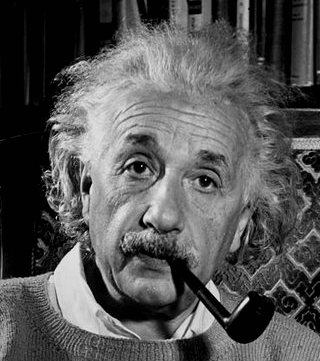
\includegraphics[width=6cm, height=6cm]{orgi/gae.jpg}
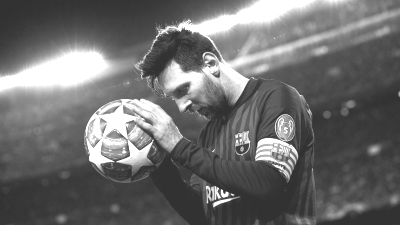
\includegraphics[width=6cm, height=6cm]{orgi/gMessi.jpg}
\caption{Obrazy wejściowe (od lewej): obraz 1 (320x361), obraz 2 (400x225) }
\end{figure}
\begin{figure}[h]
\centering
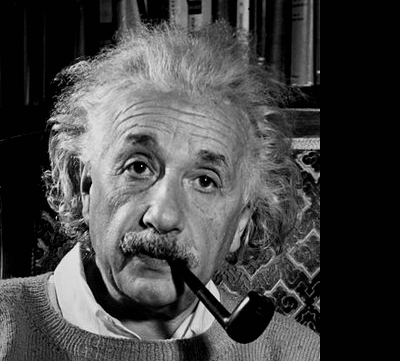
\includegraphics[width=6cm, height=6cm]{2_1/GeoG1.jpg}
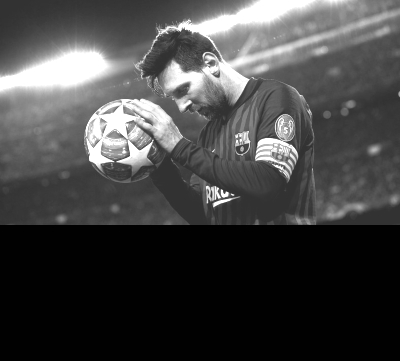
\includegraphics[width=6cm, height=6cm]{2_1/GeoG2.jpg}
\caption{Obrazy wyjściowe (od lewej): obraz 1 (400x361), obraz 2 (400x361) }
\end{figure}

\newpage
\begin{figure}[h]
\centering
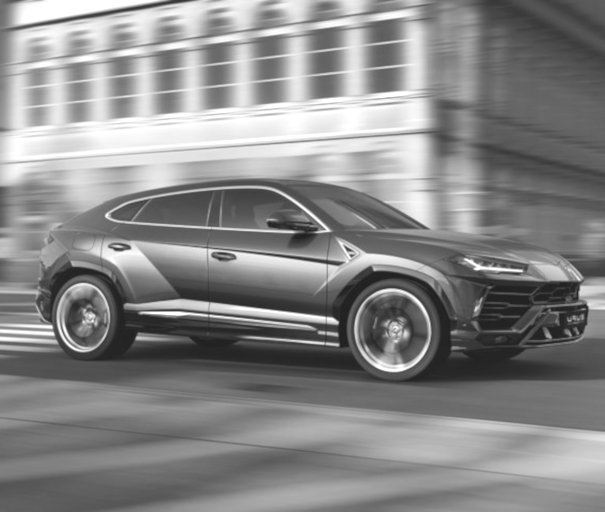
\includegraphics[width=6cm, height=6cm]{orgi/gLU.jpg}
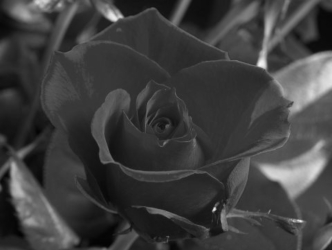
\includegraphics[width=6cm, height=6cm]{orgi/groza.jpg}
\caption{Obrazy wejściowe (od lewej): obraz 1 (605x512), obraz 2 (332x250) }
\end{figure}
\begin{figure}[h]
\centering
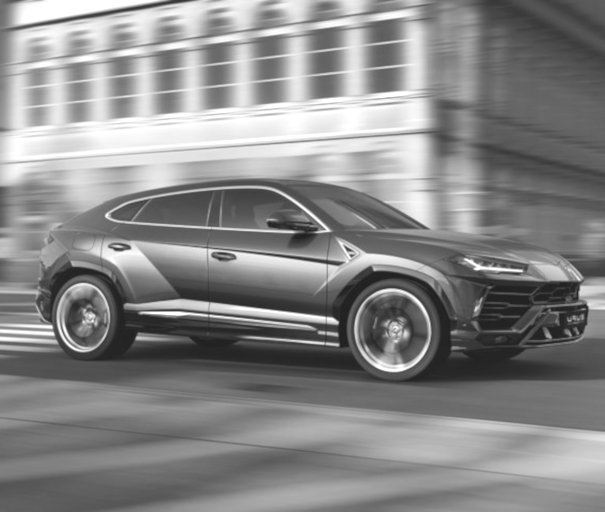
\includegraphics[width=6cm, height=6cm]{2_1/GeoG3.jpg}
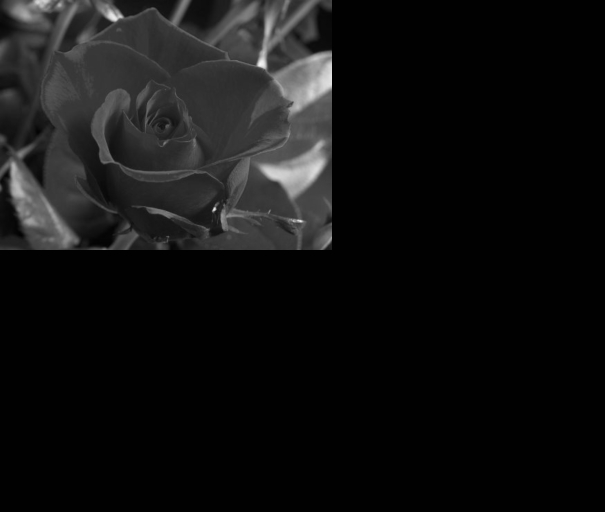
\includegraphics[width=6cm, height=6cm]{2_1/GeoG4.jpg}
\caption{Obrazy wyjściowe (od lewej): obraz 1 (605x512), obraz 2 (605x512) }
\end{figure}

\newpage
\textbf{\Large Kod funkcji}
   
\lstset{language=Python}
\vspace{0.25cm}
\begin{lstlisting}[caption={Geometryczne ujednolicanie obrazów szarych}]

def unification_Grayscale_Geometric(image1, image2):

    if (image1.imageColor == 0 or image1.imageColor == 1) and 
    (image2.imageColor == 0 or image2.imageColor == 1):

        # Dodanie i wypelnienie roznice pikselami o wartosci 1 
        w obrazie 2, ktory ma mniejsza wysokosc.
        if image1.imageLength > image2.imageLength:
            print("Dlugosc obrazu 1 jest wieksza.")

            for i in range(image2.imageLength, image1.imageLength):
                image2.imageData.append([[1]])
                for j in range(image2.imageWidth-1):
                    image2.imageData[i].append([1])

            image2.imageLength = image1.imageLength

        else:
            # Dodanie i wypelnienie roznice pikselami o wartosci 1 
            w obrazie 1, ktory ma mniejsza wysokosc.
            if image1.imageLength < image2.imageLength:
                print("Dlugosc obrazu 2 jest wieksza.")

                for i in range(image1.imageLength, image2.imageLength):
                    image1.imageData.append([[1]])
                    for j in range(image1.imageWidth-1):
                        image1.imageData[i].append([1])

                image1.imageLength = image2.imageLength

            else:
                print("Dlugosc obrazu 1 i 2 jest rowna.")

        # Dodanie i wypelnienie roznice pikselami o wartosci 1 
        w obrazie 2, ktory ma mniejsza szerokosc.
        if image1.imageWidth > image2.imageWidth:
            print("Szerokosc obrazu 1 jest wieksza.")

            for i in range(image2.imageLength):
                for j in range(image2.imageWidth, image1.imageWidth):
                    image2.imageData[i].append([1])

            image2.imageWidth = image1.imageWidth

        else:
            # Dodanie i wypelnienie roznice pikselami o wartosci 1 
            w obrazie 1, ktory ma mniejsza szerokosc.
            if image1.imageWidth < image2.imageWidth:
                print("Szerokosc obrazu 2 jest wieksza.")

                for i in range(image1.imageLength):
                    for j in range(image1.imageWidth, image2.imageWidth):
                        image1.imageData[i].append([1])

                image1.imageWidth = image2.imageWidth

            else:
                print("Szerokosc obrazu 1 i 2 jest rowna.")
    else:
        raise Exception("Ta funkcja sluzy do ujednolicenia geometrycznie 
        obrazow SZARYCH, a ktorys obraz jest RGB.")

\end{lstlisting}
\newpage

\section{Ujednolicenie obrazów szarych rozdzielczościowe}

\vspace{0.5cm}\textbf{\Large Opis ćwiczenia}
\vspace{0.25cm}\newline
Algorytm rozdzielczościowego ujednolicenia obrazów następuje po ujednoliceniu
geometrycznym i polega na doprowadzenie obydwóch obrazów do takie samej interpretacji fotometrycznej, głębi kolorów.
\newline
\newline
\textbf{\Large Opis realizowanych operacji}
\begin{enumerate}
\item Doprowadź obydwa obrazy do takiej samej interpolacji fonetycznej.
\item Doprowadź obydwa obrazy do takiej samej głębi kolorów.
%\item Zinterpolowanie większego obrazu algorytmem interpolacji dwuliniowej, każdy piksel obrazu wynikowego przyjmuje wartość na podstawie wartości czterech sąsiednich punktów obrazu wejściowego.
\end{enumerate}

\vspace{0.5cm}
\textbf{\Large Kod do wykonania danego problemu}
\lstset{language=Python}
\vspace{0.25cm}
\begin{lstlisting}
	nameFIleONE = 'img/gae.tif'
	nameFileTWO = 'img/gMessi.tif'
	readFileOne = ReadTiff(nameFIleONE)
	imageOne = Image(readFileOne)
	readFileTwo = ReadTiff(nameFileTWO)
	imageTwo = Image(readFileTwo)
	unification_Grayscale_Resolution(imageOne, imageTwo)
	writeTiff("Resolution_GRAY_3", imageOne)
	writeTiff("Resolution_GRAY_4", imageTwo)

	nameFIleTHREE = 'img/gLU.tif'
	nameFileFOUR = 'img/groza.tif'
	readFileThree = ReadTiff(nameFIleTHREE)
	imageThree = Image(readFileThree)
	readFileFour = ReadTiff(nameFileFOUR)
	imageFour = Image(readFileFour)
	unification_Grayscale_Resolution(imageThree, imageFour)
	writeTiff("Resolution_GRAY_3", imageThree)
	writeTiff("Resolution_GRAY_4", imageFour)

\end{lstlisting}

\newpage
\vspace{0.25cm}\textbf{\Large Przeprowadzone testy}
\vspace{0.5cm}
\begin{figure}[h]
\centering
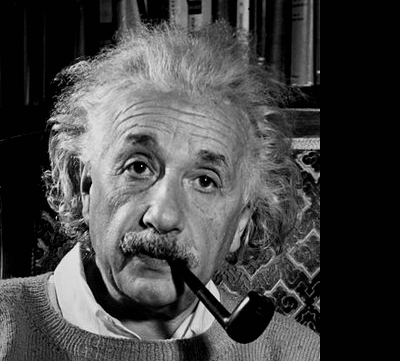
\includegraphics[width=6cm, height=6cm]{2_1/GeoG1.jpg}
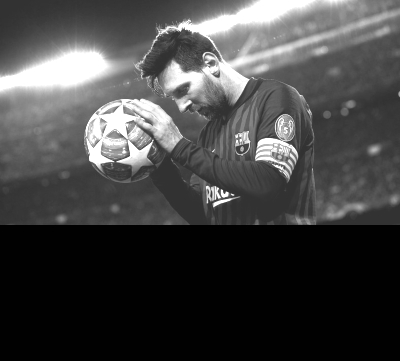
\includegraphics[width=6cm, height=6cm]{2_1/GeoG2.jpg}
\caption{Obrazy wejściowe (od lewej): obraz 1 (400x361), obraz 2 (400x361) }
\end{figure}
\begin{figure}[h]
\centering
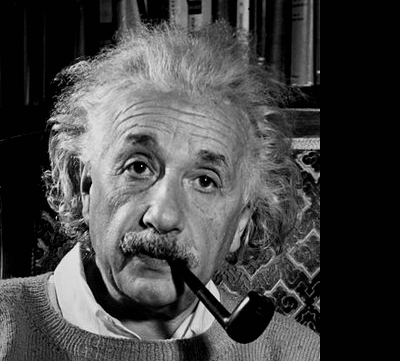
\includegraphics[width=6cm, height=6cm]{2_2/ResolG1.jpg}
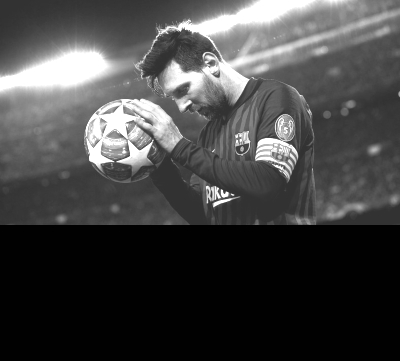
\includegraphics[width=6cm, height=6cm]{2_2/ResolG2.jpg}
\caption{Obrazy wyjściowe (od lewej): obraz 1 (400x361), obraz 2 (400x361) }
\end{figure}

\newpage
\begin{figure}[h]
\centering
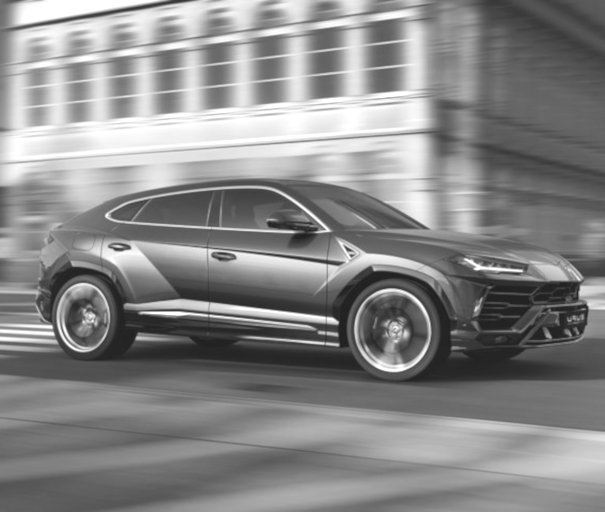
\includegraphics[width=6cm, height=6cm]{2_1/GeoG3.jpg}
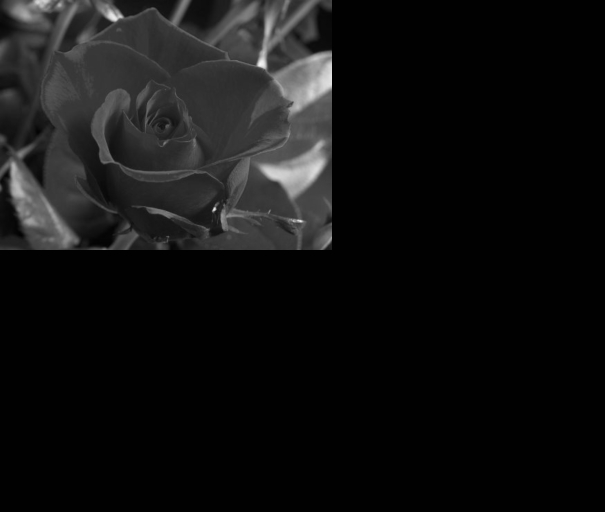
\includegraphics[width=6cm, height=6cm]{2_1/GeoG4.jpg}
\caption{Obrazy wejściowe (od lewej): obraz 1 (605x512), obraz 2 (605x512) }
\end{figure}
\begin{figure}[h]
\centering
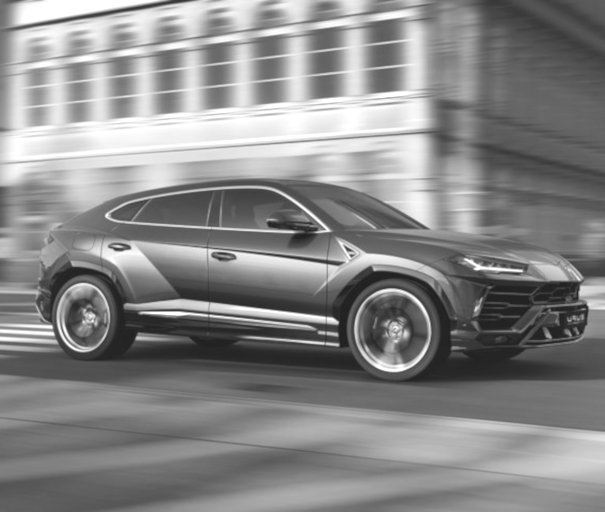
\includegraphics[width=6cm, height=6cm]{2_2/ResolG3.jpg}
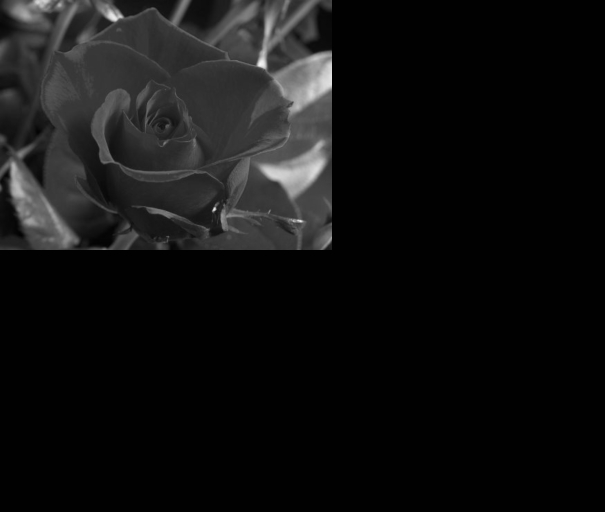
\includegraphics[width=6cm, height=6cm]{2_2/ResolG4.jpg}
\caption{Obrazy wyjściowe (od lewej): obraz 1 (605x512), obraz 2 (605x512) }
\end{figure}

\newpage
\textbf{\Large Kod funkcji}
   
\lstset{language=Python}
\vspace{0.25cm}
\begin{lstlisting}[caption={Rozdzielczościowe ujednolicanie obrazów szarych}]

def unification_Grayscale_Resolution(image1, image2):
   
    if (image1.imageColor == 0 or image1.imageColor == 1) and 
    (image2.imageColor == 0 or image2.imageColor == 1):

        # Doprowadzenie obydwoch obrazow do takiej samej glebi kolorow
        if image1.imageBitsColor[0] != image2.imageBitsColor[0]:

            if image1.imageBitsColor[0] == 4:
                print("Zmiana rozdzielczosci obrazu 1 z 4 na 8 bitow.")
                for i in range(image1.imageLength):
                    for j in range(image1.imageWidth):
                        image1.imageData[i][j][0] = 
                        image1.imageData[i][j][0] * 16
                image1.imageBitsColor[0] = 8

                for i in range(image1.originalImageLength):
                    for j in range(image1.originalImageWidth):
                        image1.originalImageData[i][j][0] =
                         image1.originalImageData[i][j][0] * 16

            else:
                print("Zmiana rozdzielczosci obrazu 2 z 4 na 8 bitow.")
                if image2.imageBitsColor[0] == 4:
                    for i in range(image2.imageLength):
                        for j in range(image2.imageWidth):
                            image2.imageData[i][j][0] = 
                            image2.imageData[i][j][0] * 16
                    image2.imageBitsColor[0] = 8

                    for i in range(image2.originalImageLength):
                        for j in range(image2.originalImageWidth):
                            image2.originalImageData[i][j][0] =
                             image2.originalImageData[i][j][0] * 16

                else:
                    raise Exception("programu 3")

        else:
            print("Rozdzielczosc obrazow 1 i 2 SZARYCH jest taka sama.")

        # Doprowadzenie obydwoch obrazow do takiej samej 
        interpretacji fotometrycznej
        if image1.imageColor != image2.imageColor:

            if image1.imageColor == 0:
                if image1.imageBitsColor[0] == 8:
                    for i in range(image1.imageLength):
                        for j in range(image1.imageWidth):
                            image1.imageData[i][j][0] = 
                            255 - image1.imageData[i][j][0]

                    for i in range(image1.originalImageLength):
                        for j in range(image1.originalImageWidth):
                            image1.originalImageData[i][j][0] = 
                            255 - image1.originalImageData[i][j][0]

                else:
                    if image1.imageBitsColor[0] == 4:
                        for i in range(image1.imageLength):
                            for j in range(image1.imageWidth):
                                image1.imageData[i][j][0] =
                                 15 - image1.imageData[i][j][0]

                        for i in range(image1.originalImageLength):
                            for j in range(image1.originalImageWidth):
                                image1.originalImageData[i][j][0] =
                                 15 - image1.originalImageData[i][j][0]

                    else:
                        raise Exception("programu 4")
                image1.imageColor = 1

            else:
                if image2.imageColor == 0:
                    if image2.imageBitsColor[0] == 8:
                        for i in range(image2.imageLength):
                            for j in range(image2.imageWidth):
                                image2.imageData[i][j][0] =
                                255 - image2.imageData[i][j][0]

                        for i in range(image2.originalImageLength):
                            for j in range(image2.originalImageWidth):
                                image2.originalImageData[i][j][0] =
                                255 -image2.originalImageData[i][j][0]

                    else:
                        if image2.imageBitsColor[0] == 4:
                            for i in range(image2.imageLength):
                                for j in range(image2.imageWidth):
                                    image2.imageData[i][j][0] = 
                                    15 -image2.imageData[i][j][0]

                            for i in range(image2.originalImageLength):
                                for j in range(image2.originalImageWidth):
                                    image2.originalImageData[i][j][0] = 
                                    15 - image2.originalImageData[i][j][0]

                        else:
                            raise Exception("programu 5")
                    image2.imageColor = 1
                else:
                    raise Exception("programu 6")
        else:
            print("Kolor obrazy maja taki sam.")

    else:
        raise Exception("Ta funkcja sluzy do ujednolicenia rozdzielczosciowo
        obrazow SZARYCH, a ktorys obraz jest RGB.")

\end{lstlisting}
\newpage

\section{Ujednolicenie obrazów RGB geometryczne}

\vspace{0.5cm}\textbf{\Large Opis ćwiczenia}
\vspace{0.25cm}\newline
Algorytm geometrycznego ujednolicenia obrazów polega na doprowadzeniu z mniejszymi rozmiarami obrazu do większego rozmiarami obrazu, czyli doprowadzenie obrazów do takiej samej liczby wierszy i kolumn piksli w każdym obrazie.
Ten sposób ujednolicania nie powoduje spadku jakości obrazów.
\newline
\newline
\textbf{\Large Opis realizowanych operacji}
\begin{enumerate}
\item Wybierz największą szerokość i największą wysokość z dwóch obrazów.
\item Dodaj i wypełni różnicę pikselami o wartości 1 dla każdego z kanałów w obrazie, który ma mniejszą szerokość albo wysokość.
%\item Umieść obrazek na środku macierzy w powiększonym obrazie 
\end{enumerate}

\vspace{0.5cm}
\textbf{\Large Kod do wykonania danego problemu}
\lstset{language=Python}
\vspace{0.25cm}
\begin{lstlisting}
	nameFIleONE = 'img/RGBMessi.tif'
	nameFileTWO = 'img/RGBLL.tif'
	readFileOne = ReadTiff(nameFIleONE)
	imageOne = Image(readFileOne)
	readFileTwo = ReadTiff(nameFileTWO)
	imageTwo = Image(readFileTwo)
	unification_RGB_Geometric(imageOne, imageTwo)
	writeTiff("Geometric_RGB_1", imageOne)
	writeTiff("Geometric_RGB_2", imageTwo)
    
	nameFIleTHREE = 'img/RGBkamel.tif'
	nameFileFOUR = 'img/RGBkulki.tif'
	readFileThree = ReadTiff(nameFIleTHREE)
	imageThree = Image(readFileThree)
	readFileFour = ReadTiff(nameFileFOUR)
	imageFour = Image(readFileFour)
	unification_RGB_Geometric(imageThree, imageFour)
	writeTiff("Geometric_RGB_3", imageThree)
	writeTiff("Geometric_RGB_4", imageFour)

\end{lstlisting}

\newpage
\vspace{0.25cm}\textbf{\Large Przeprowadzone testy}
\vspace{0.5cm}
\begin{figure}[h]
\centering
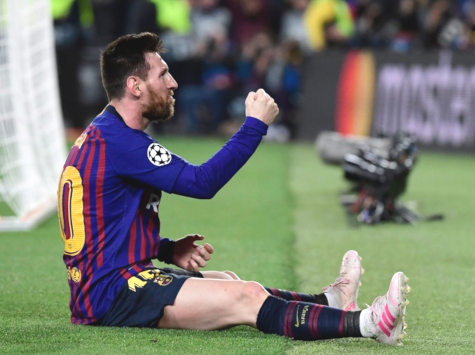
\includegraphics[width=6cm, height=6cm]{orgi/RGBMessi.jpg}
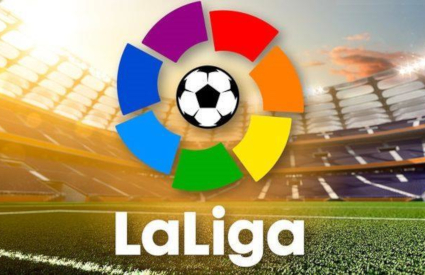
\includegraphics[width=6cm, height=6cm]{orgi/RGBLL.jpg}
\caption{Obrazy wejściowe (od lewej): obraz 1 (475x355), obraz 2 (425x275) }
\end{figure}
\begin{figure}[h]
\centering
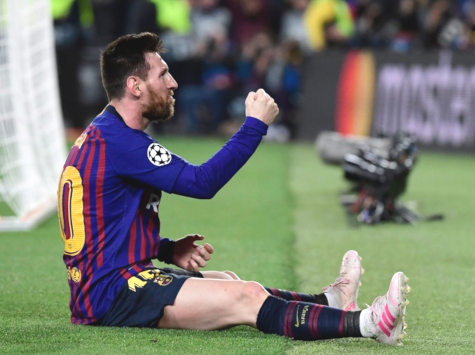
\includegraphics[width=6cm, height=6cm]{2_3/GeoRGB1.jpg}

\includegraphics[width=6cm, height=6cm]{2_3/GeoRGB2.jpg}
\caption{Obrazy wyjściowe (od lewej): obraz 1 (475x355), obraz 2 (475x355) }
\end{figure}

\newpage
\begin{figure}[h]
\centering
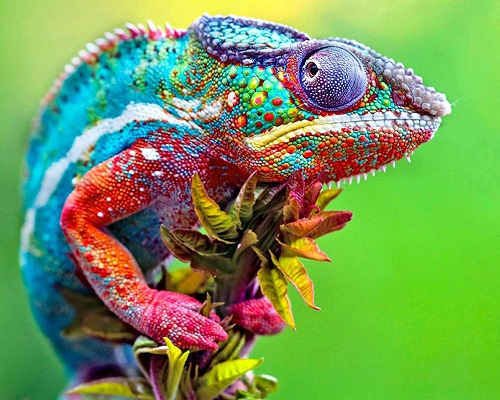
\includegraphics[width=6cm, height=6cm]{orgi/RGBkamel.jpg}
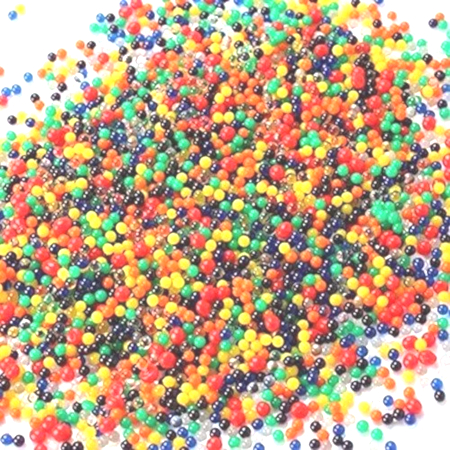
\includegraphics[width=6cm, height=6cm]{orgi/RGBkulki.jpg}
\caption{Obrazy wejściowe (od lewej): obraz 1 (500x400), obraz 2 (450x450) }
\end{figure}
\begin{figure}[h]
\centering
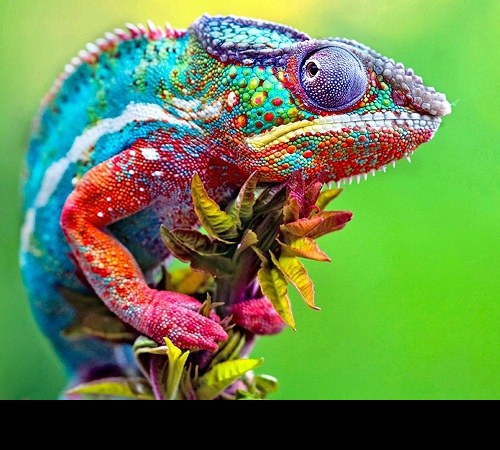
\includegraphics[width=6cm, height=6cm]{2_3/GeoRGB3.jpg}
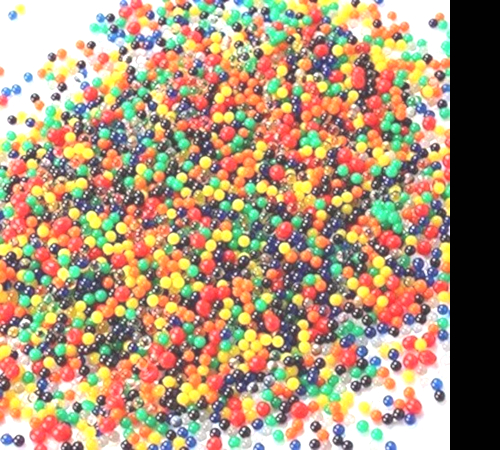
\includegraphics[width=6cm, height=6cm]{2_3/GeoRGB4.jpg}
\caption{Obrazy wyjściowe (od lewej): obraz 1 (500x450), obraz 2 (500x450) }
\end{figure}

\newpage
\textbf{\Large Kod funkcji}
   
\lstset{language=Python}
\vspace{0.25cm}
\begin{lstlisting}[caption={Geometryczne ujednolicanie obrazów RGB}]


def unification_RGB_Geometric(image1, image2):

    if image1.imageColor == 2 and image2.imageColor == 2:

        # Dodanie i wypelnienie roznice pikselami o wartosci 1 w obrazie 2,
         ktory ma mniejsza wysokosc.
        if image1.imageLength > image2.imageLength:
            print("Dlugosc obrazu 1 jest wieksza.")

            for i in range(image2.imageLength, image1.imageLength):
                image2.imageData.append([[1, 1, 1]])
                for j in range(image2.imageWidth-1):
                    image2.imageData[i].append([1, 1, 1])
            image2.imageLength = image1.imageLength

        else:
            # Dodanie i wypelnienie roznice pikselami o wartosci 1 w obrazie 1,
            ktory ma mniejsza wysokosc.
            if image1.imageLength < image2.imageLength:
                print("Dlugosc obrazu 2 jest wieksza.")

                for i in range(image1.imageLength, image2.imageLength):
                    image1.imageData.append([[1, 1, 1]])
                    for j in range(image1.imageWidth-1):
                        image1.imageData[i].append([1, 1, 1])
                image1.imageLength = image2.imageLength

            else:
                print("Dlugosc obrazu 1 i 2 jest rowna.")

        # Dodanie i wypelnienie roznice pikselami o wartosci 1 w obrazie 2,
         ktory ma mniejsza szerokosc.
        if image1.imageWidth > image2.imageWidth:
            print("Szerokosc obrazu 1 jest wieksza.")

            for i in range(image2.imageLength):
                for j in range(image2.imageWidth, image1.imageWidth):
                    image2.imageData[i].append([1, 1, 1])
            image2.imageWidth = image1.imageWidth

        else:
            # Dodanie i wypelnienie roznice pikselami o wartosci 1 w obrazie 1,
             ktory ma mniejsza szerokosc.
            if image1.imageWidth < image2.imageWidth:
                print("Szerokosc obrazu 2 jest wieksza.")

                for i in range(image1.imageLength):
                    for j in range(image1.imageWidth, image2.imageWidth):
                        image1.imageData[i].append([1, 1, 1])
                image1.imageWidth = image2.imageWidth

            else:
                print("Szerokosc obrazu 1 i 2 jest rowna.")

    else:
        raise Exception("Ta funkcja sluzy do ujednolicenia geometrycznie
         obrazow RGB, a ktorys obraz jest SZARY.")

\end{lstlisting}
\newpage


\section{Ujednolicenie obrazów RGB rozdzielczościowe}

\vspace{0.5cm}\textbf{\Large Opis ćwiczenia}
\vspace{0.25cm}\newline
Algorytm rozdzielczościowego ujednolicenia obrazów następuje po ujednoliceniu
geometrycznym i polega na doprowadzenie obydwóch obrazów do takie samej interpretacji fotometrycznej, głębi kolorów.
\newline
\newline
\textbf{\Large Opis realizowanych operacji}
\begin{enumerate}
\item Doprowadź obydwa obrazy do takiej samej interpolacji fonetycznej.
\item Doprowadź obydwa obrazy do takiej samej głębi kolorów.
%\item Zinterpolowanie większego obrazu, algorytmem interpolacji dwuliniowej, każdy piksel obrazu wynikowego przyjmuje wartość na podstawie wartości czterech sąsiednich punktów obrazu wejściowego.
\end{enumerate}

\vspace{0.5cm}
\textbf{\Large Kod do wykonania danego problemu}
\lstset{language=Python}
\vspace{0.25cm}
\begin{lstlisting}
	nameFIleONE = 'img/RGBMessi.tif'
	nameFileTWO = 'img/RGBLL.tif'
	readFileOne = ReadTiff(nameFIleONE)
	imageOne = Image(readFileOne)
	readFileTwo = ReadTiff(nameFileTWO)
	imageTwo = Image(readFileTwo)
	unification_RGB_Resolution(imageOne, imageTwo)
	writeTiff("Resolution_RGB_1", imageOne)
	writeTiff("Resolution_RGB_2", imageTwo)
	
	nameFIleTHREE = 'img/RGBkamel.tif'
	nameFileFOUR = 'img/RGBkulki.tif'
	readFileThree = ReadTiff(nameFIleTHREE)
	imageThree = Image(readFileThree)
	readFileFour = ReadTiff(nameFileFOUR)
	imageFour = Image(readFileFour)
	unification_RGB_Resolution(imageThree, imageFour)
	writeTiff("Resolution_RGB_3", imageThree)
	writeTiff("Resolution_RGB_4", imageFour)

\end{lstlisting}

\newpage
\vspace{0.25cm}\textbf{\Large Przeprowadzone testy}
\vspace{0.5cm}
\begin{figure}[h]
\centering
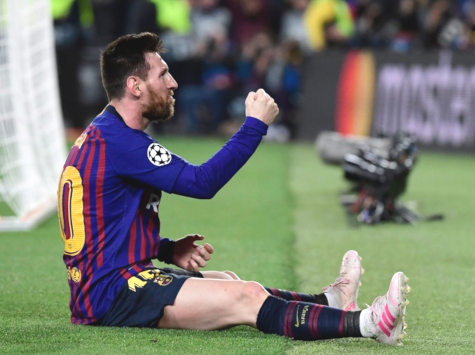
\includegraphics[width=6cm, height=6cm]{2_3/GeoRGB1.jpg}

\includegraphics[width=6cm, height=6cm]{2_3/GeoRGB2.jpg}
\caption{Obrazy wejściowe (od lewej): obraz 1 (475x355), obraz 2 (475x355) }
\end{figure}
\begin{figure}[h]
\centering
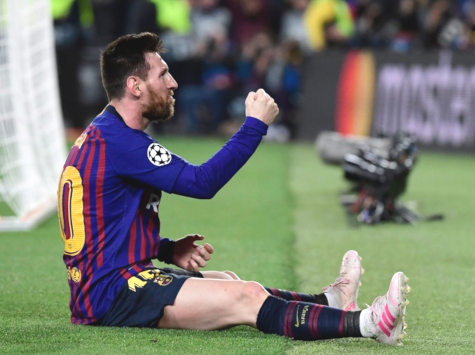
\includegraphics[width=6cm, height=6cm]{2_4/ResolRGB1.jpg}

\includegraphics[width=6cm, height=6cm]{2_4/ResolRGB2.jpg}
\caption{Obrazy wyjściowe (od lewej): obraz 1 (475x355), obraz 2 (475x355) }
\end{figure}

\newpage
\begin{figure}[h]
\centering
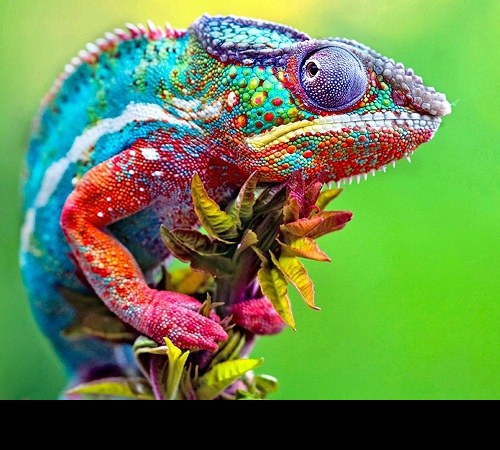
\includegraphics[width=6cm, height=6cm]{2_3/GeoRGB3.jpg}
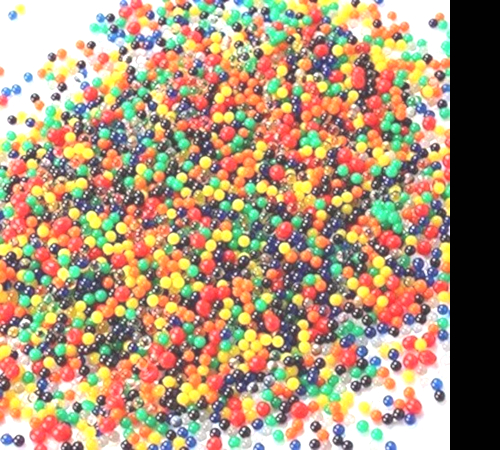
\includegraphics[width=6cm, height=6cm]{2_3/GeoRGB4.jpg}
\caption{Obrazy wejściowe (od lewej): obraz 1 (500x450), obraz 2 (500x450) }
\end{figure}
\begin{figure}[h]
\centering
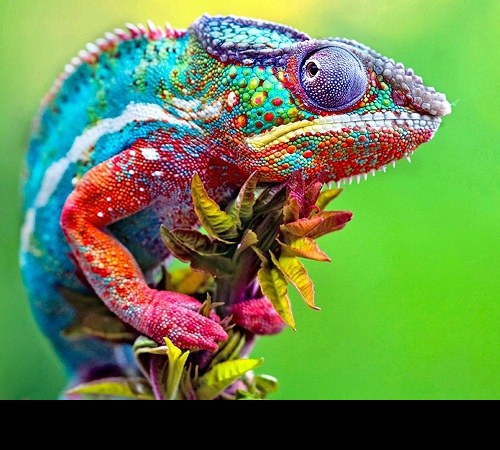
\includegraphics[width=6cm, height=6cm]{2_4/ResolRGB3.jpg}
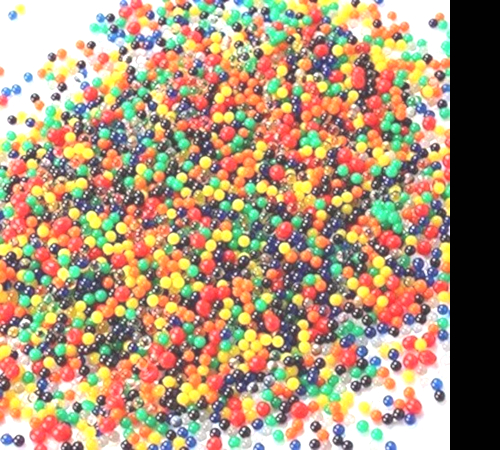
\includegraphics[width=6cm, height=6cm]{2_4/ResolRGB4.jpg}
\caption{Obrazy wyjściowe (od lewej): obraz 1 (500x450), obraz 2 (500x450) }
\end{figure}

\newpage
\textbf{\Large Kod funkcji}
   
\lstset{language=Python}
\vspace{0.25cm}
\begin{lstlisting}[caption={Rozdzielczościowe ujednolicanie obrazów RGB}]

def unification_RGB_Resolution(image1, image2):

    if image1.imageColor == 2 and image2.imageColor == 2:

        # Doprowadzenie obydwoch obrazow do takiej samej glebi kolorow
        if image1.imageBitsColor[0] != image2.imageBitsColor[0]:

            if image1.imageBitsColor[0] == 4:
                for i in range(image1.imageLength):
                    for j in range(image1.imageWidth):
                        for k in range(3):
                            image1.imageData[i][j][k] =
                             image1.imageData[i][j][k] * 16
                for l in range(3):
                    image1.imageBitsColor[l] = 8

                for i in range(image1.originalImageLength):
                    for j in range(image1.originalImageWidth):
                        for k in range(3):
                            image1.originalImageData[i][j][k] =
                             image1.originalImageData[i][j][k] * 16

            else:
                if image2.imageBitsColor[0] == 4:
                    for i in range(image2.imageLength):
                        for j in range(image2.imageWidth):
                            for k in range(3):
                                image2.imageData[i][j][k] =
                                 image2.imageData[i][j][k] * 16
                    for l in range(3):
                        image2.imageBitsColor[l] = 8

                    for i in range(image2.originalImageLength):
                        for j in range(image2.originalImageWidth):
                            for k in range(3):
                                image2.originalImageData[i][j][k] =
                                 image2.originalImageData[i][j][k] * 16
                else:
                    raise Exception("programu 3")
        else:
            print("Rozdzielczosc obrazow 1 i 2 RGB jest taka sama.")
    else:
        raise Exception("Ta funkcja sluzy do ujednolicenia rozdzielczosciowo
         obrazow RGB, a ktorys obraz jest SZARY.")

\end{lstlisting}



\chapter{Operacje sumowania arytmetycznego obrazów szarych}
\section{Sumowanie (okreslonej) stałej z obrazem}

\vspace{0.5cm}\textbf{\Large Opis ćwiczenia}
\vspace{0.25cm}\newline
Algorytm sumowania obrazu szarego z określoną stałą polega na dodaniu do każdej
wartości
pojedynczego piksla stałej liczby. Po operacji sumowania następuje normalizacja
obrazu.
\newline
\newline
\textbf{\Large Opis realizowanych operacji}
\begin{enumerate}
\item Policz sumy wartości każdego piksla ze stałą.
\item Jeśli przynajmniej jedna z tych sum jest większa od głębi kolorów obrazu to:
\item Wybierz największą sumę $Q_{max}$ i $D_{max}$ policz ze wzoru
\newline $D_{max}[i,j]=(Q_{max}[i,j]$ - głębia koloru obrazu$)$
\item Policz proporcję $X=D_{max}[i,j]/$głębia koloru obrazu 
\newline i zaokrąglając wynik do najbliższej z góry liczby całkowitej.
\item Jeśli nie ma sumy większej od głębi kolorów obrazu to X=0.
\item Policz sumy: 
\newline $Q[i,j]=P[i,j]-(P[i,j]*X)+const-(const*X)$
\item Znormalizowanie obrazu wzorem:
\newline $f_{norm}=Z_{rep}[(f-f_{min})/(f_{max}-f_{min})]$
\end{enumerate}

\newpage
%\vspace{0.5cm}
\textbf{\Large Kod do wykonania danego problemu}
\lstset{language=Python}
\vspace{0.25cm}
\begin{lstlisting}

	nameFileTWO = 'img/gMessi.tif'
	readFileTwo = ReadTiff(nameFileTWO)
	imageTwo = Image(readFileTwo)
	sum_const_grayscale(imageTwo, 50)
    
	nameFIleTHREE = 'img/gLU.tif'
	readFileThree = ReadTiff(nameFIleTHREE)
	imageThree = Image(readFileThree)
	sum_const_grayscale(imageThree, 100)

\end{lstlisting}

%\newpage
\vspace{0.25cm}\textbf{\Large Przeprowadzone testy}
\vspace{0.5cm}
\begin{figure}[h]
\centering
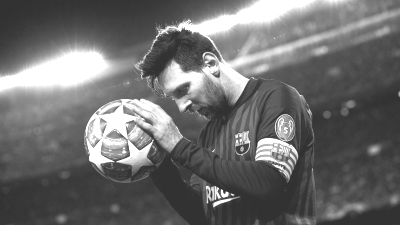
\includegraphics[width=5cm, height=5cm]{orgi/gMessi.jpg}
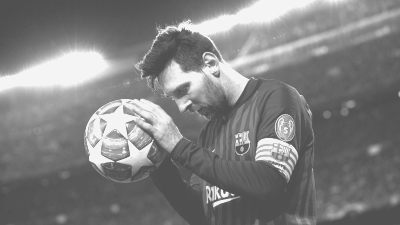
\includegraphics[width=5cm, height=5cm]{3_1/add_constG1.jpg}
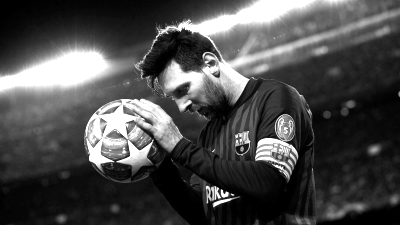
\includegraphics[width=5cm, height=5cm]{3_1/nadd_constG1.jpg}
\caption{(Od lewej): obraz wejściowy szary, obraz po sumowaniu ze stałą = 50, obraz po normalizacji}
\end{figure}
\begin{figure}[h]
\centering
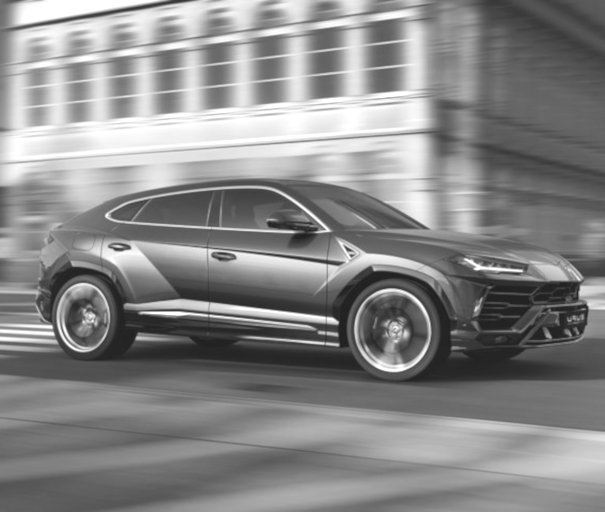
\includegraphics[width=5cm, height=5cm]{orgi/gLU.jpg}
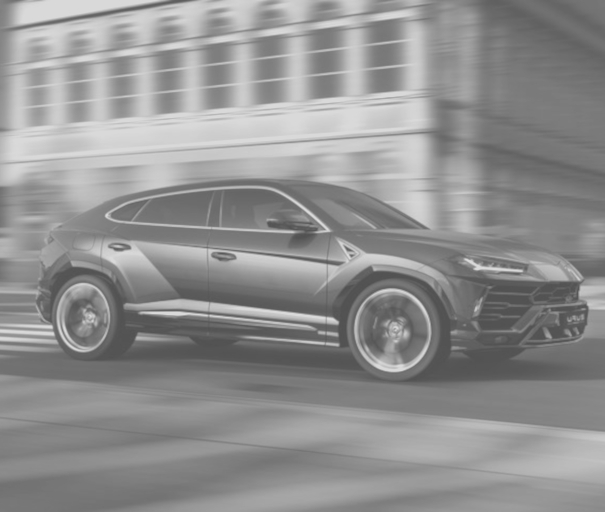
\includegraphics[width=5cm, height=5cm]{3_1/add_constG2.jpg}
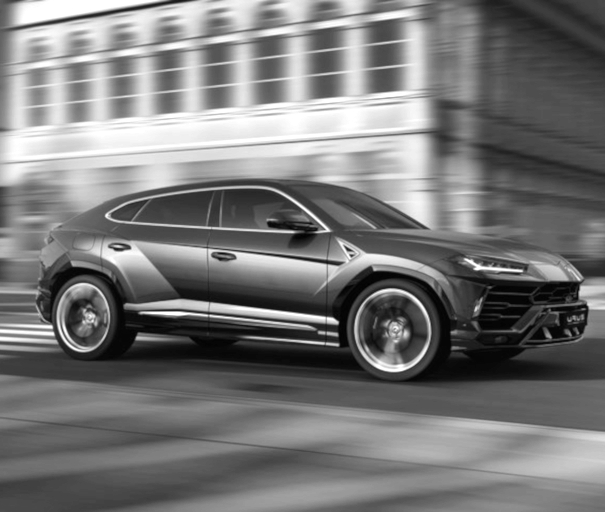
\includegraphics[width=5cm, height=5cm]{3_1/nadd_constG2.jpg}
\caption{(Od lewej): obraz wejściowy szary, obraz po sumowaniu ze stałą = 100, obraz po normalizacji}
\end{figure}

\newpage
\textbf{\Large Kod funkcji}
   
\lstset{language=Python}
\vspace{0.25cm}
\begin{lstlisting}[caption={Sumowanie (okreslonej) stałej z obrazem szarym}]

def sum_const_grayscale(image1, const=0):
    if image1.imageBitsColor[0] == 4:

        maxBitsColor = 15
        if not (0 <= const <= 15):
            raise Exception("program do obrazow SZARYCH 4 bitowych 
            mozne dodac liczbe z zakresu 0-15, a podana liczba "
                            "to %d." % const)
    else:
        if image1.imageBitsColor[0] == 8:

            maxBitsColor = 255
            if not (0 <= const <= 255):
                raise Exception("program do obrazow SZARYCH 8 bitowych 
                mozne dodac liczbe z zakresu 0-255, a podana "
                                "podana to %d." % const)
        else:
            raise Exception("program dodaje jedynie obrazy SZARE 4, 8 bitowe
            ze stala")

    Qmax = 0
    Dmax = 0
    X = 0
    fmax = 0
    fmin = 256

    for i in range(image1.imageLength):
        for j in range(image1.imageWidth):

            # obliczanie sumy obrazu z stala
            temp = image1.imageData[i][j][0] + const

            # poszukiwanie maksimum w obrazie
            if temp > Qmax:
                Qmax = temp

    # sprawdzenie, czy maksimum obrazu przekracza zakres
    if Qmax > maxBitsColor:
        Dmax = Qmax - maxBitsColor
        X = round(Dmax/maxBitsColor, 2)

    if X == 1.0:
        X = 0.99

    # dodawanie obrazu ze stala z uzwglenieniem zakresu
    for i in range(image1.imageLength):
        for j in range(image1.imageWidth):
            tempSum = ceil((image1.imageData[i][j][0] -
             (image1.imageData[i][j][0] * X)) + (const - (const * X)))
            image1.imageData[i][j][0] = tempSum

            # poszukiwanie maksimum
            if tempSum > fmax:
                fmax = tempSum

            # poszukiwanie minimum
            if tempSum < fmin:
                fmin = tempSum

    writeTiff('add_const', image1)

    # normalizacja
    for i in range(image1.imageLength):
        for j in range(image1.imageWidth):
            image1.imageData[i][j][0] = round(maxBitsColor *
             ((image1.imageData[i][j][0] - fmin) / (fmax - fmin)))
    writeTiff('normalization_add_const', image1)

\end{lstlisting}


\newpage
\section{Sumowanie dwóch obrazów}

\vspace{0.5cm}\textbf{\Large Opis ćwiczenia}
\vspace{0.25cm}\newline
Algebraiczne sumowanie obrazów f i f’ jest określone jedynie dla obrazów o tych samych wymiarach M x N i strukturze ich macierzy. Algorytm sumowania obrazu z obrazem polega na dodaniu do wartości piksla z pierwszego obrazu, wartości odpowiadającego piksla z drugiego obrazu. Po operacji sumowania następuje normalizacja obrazu. Dodawanie obrazów jest użyteczne w uśrednianiu obrazów, wykonywanym w celu zredukowania na nich szumu.
\newline
\newline
\textbf{\Large Opis realizowanych operacji}
\begin{enumerate}
\item Policz sumy dla wszystkich piksli, odpowiadających składowych barw.
\item Jeśli przynajmniej jedna z tych sum jest większa od głębi kolorów obrazu to:
\item Wybierz największą sumę $Q_{max}$ i $D_{max}$ policz ze wzoru
\newline $D_{max}[i,j]=(Q_{max}[i,j]$ - głębia koloru obrazu$)$
\item Policz proporcję $X=D_{max}[i,j]/$głębia koloru obrazu 
\newline i zaokrąglając wynik do najbliższej z góry liczby całkowitej.
\item Jeśli nie ma sumy większej od głębi kolorów obrazu to X=0.
\item Policz sumy: 
\newline $Q[i,j]=P1[i,j]-(P1[i,j]*X)+P2[i,j]-(P2[i,j]*X)$
\item Znormalizowanie obrazu wzorem:
\newline $f_{norm}=Z_{rep}[(f-f_{min})/(f_{max}-f_{min})]$
\end{enumerate}

\vspace{0.5cm}
\textbf{\Large Kod do wykonania danego problemu}
\lstset{language=Python}
\vspace{0.25cm}
\begin{lstlisting}
	nameFIleONE = 'img/gae.tif'
	nameFileTWO = 'img/gMessi.tif'
	readFileOne = ReadTiff(nameFIleONE)
	imageOne = Image(readFileOne)
	readFileTwo = ReadTiff(nameFileTWO)
	imageTwo = Image(readFileTwo)
	unification_Grayscale_Geometric(imageOne, imageTwo)
	unification_Grayscale_Resolution(imageOne, imageTwo) 
	sum_two_images_grayscale(imageOne, imageTwo)
	nameFIleTHREE = 'img/gLU.tif'
	nameFileFOUR = 'img/groza.tif'
	readFileThree = ReadTiff(nameFIleTHREE)
	imageThree = Image(readFileThree)
	readFileFour = ReadTiff(nameFileFOUR)
	imageFour = Image(readFileFour)
	unification_Grayscale_Geometric(imageThree, imageFour)
	unification_Grayscale_Resolution(imageThree, imageFour)
	sum_two_images_grayscale(imageThree,imageFour)

\end{lstlisting}


\newpage
\vspace{0.25cm}\textbf{\Large Przeprowadzone testy}
\vspace{0.5cm}
\begin{figure}[h]
\centering
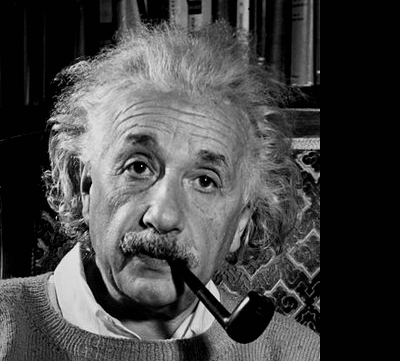
\includegraphics[width=6cm, height=6cm]{2_2/ResolG1.jpg}
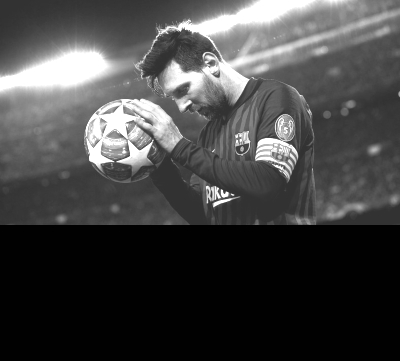
\includegraphics[width=6cm, height=6cm]{2_2/ResolG2.jpg}
\caption{Obrazy wejściowe (od lewej):pierwszy obraz wejściowy,drugi obraz wejściowy}
\end{figure}
\begin{figure}[h]
\centering
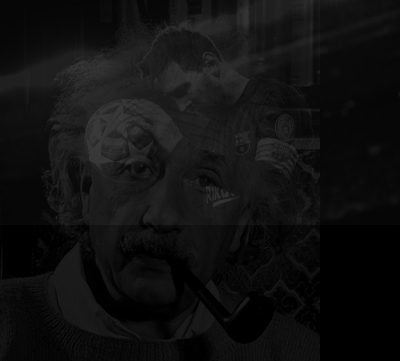
\includegraphics[width=6cm, height=6cm]{3_2/add_twoG1.jpg}
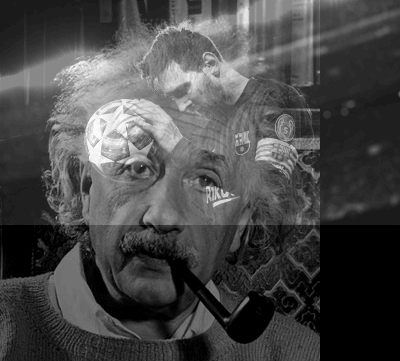
\includegraphics[width=6cm, height=6cm]{3_2/nadd_twoG1.jpg}
\caption{Obrazy wyjściowe (od lewej): obraz powstały w wyniku sumowania dwóch obrazów, obraz wynikowy po normalizacji}
\end{figure}

\newpage
\begin{figure}[h]
\centering
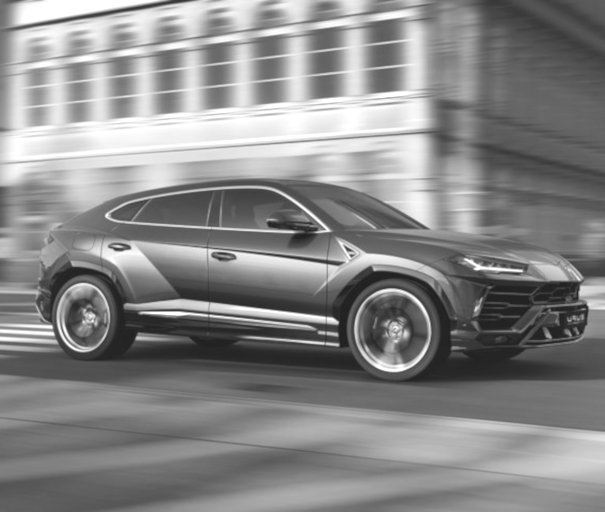
\includegraphics[width=6cm, height=6cm]{2_2/ResolG3.jpg}
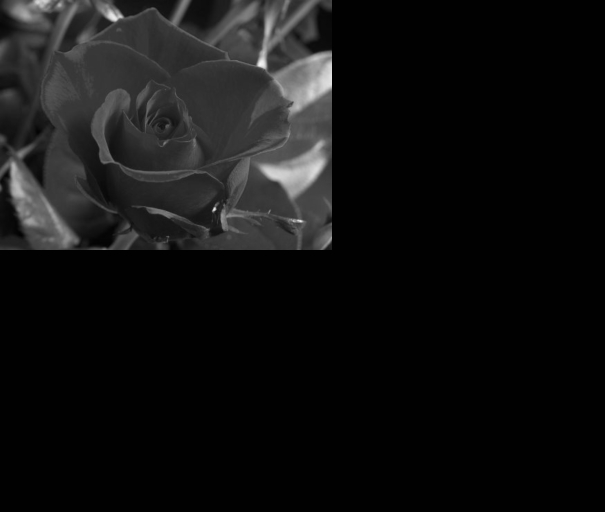
\includegraphics[width=6cm, height=6cm]{2_2/ResolG4.jpg}
\caption{Obrazy wejściowe (od lewej):pierwszy obraz wejściowy,drugi obraz wejściowy}
\end{figure}
\begin{figure}[h]
\centering
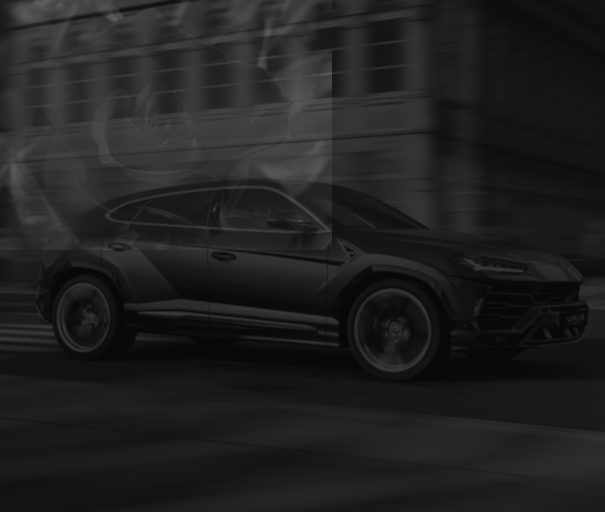
\includegraphics[width=6cm, height=6cm]{3_2/add_twoG2.jpg}
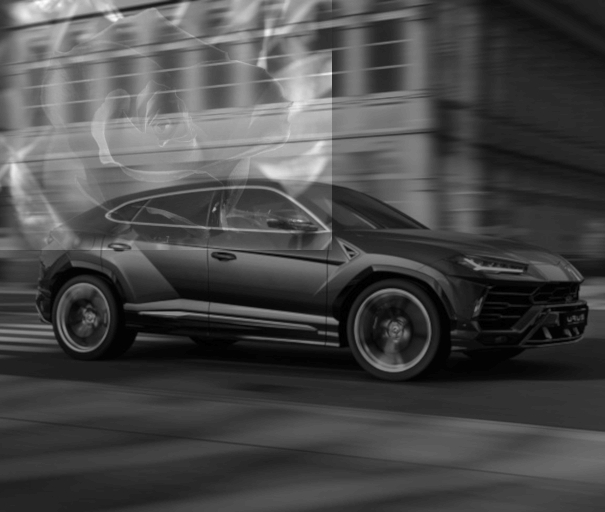
\includegraphics[width=6cm, height=6cm]{3_2/nadd_twoG2.jpg}
\caption{Obrazy wyjściowe (od lewej): obraz powstały w wyniku sumowania dwóch obrazów, obraz wynikowy po normalizacji}
\end{figure}

\newpage
\textbf{\Large Kod funkcji}
   
\lstset{language=Python}
\vspace{0.25cm}
\begin{lstlisting}[caption={Sumowanie dwóch obrazów szarych}]

def sum_two_images_grayscale(image1, image2):

    global maxBitsColor
    if image1.imageBitsColor[0] == image2.imageBitsColor[0] and
     (image1.imageLength == image2.imageLength) and 
     (image1.imageWidth == image2.imageWidth):

        if image1.imageBitsColor[0] == 4:
            maxBitsColor = 15

        else:
            if image1.imageBitsColor[0] == 8:
                maxBitsColor = 255

    else:
        raise Exception("program dodaje jedynie obrazy SZARE 4, 8 bitowe
         oraz obrazy musza miec takie same rozmiary.")

    Qmax = 0
    Dmax = 0
    X = 0
    fmax = 0
    fmin = 256

    # obliczanie sumy dwoch obrazow
    for i in range(image1.imageLength):
        for j in range(image1.imageWidth):
            temp = image1.imageData[i][j][0] + image2.imageData[i][j][0]

            # poszukiwanie maksimum w sumie obrazow
            if temp > Qmax:
                Qmax = temp

    # sprawdzenie, czy maksimum sumowanego obrazu przekracza zakres
    if Qmax > maxBitsColor:
        Dmax = Qmax - maxBitsColor
        X = round(Dmax/maxBitsColor, 2)

    if X == 1.0:
        X = 0.99

    # dodawanie dwoch obrazu  z uzwglenieniem zakresu
    for i in range(image1.imageLength):
        for j in range(image1.imageWidth):
            tempSum = round((image1.imageData[i][j][0] - 
            (image1.imageData[i][j][0] * X)) + 
            (image2.imageData[i][j][0] - (image2.imageData[i][j][0] * X)))
            image1.imageData[i][j][0] = tempSum

            # poszukiwanie maksimum
            if tempSum > fmax:
                fmax = tempSum

            # poszukiwanie minimum
            if tempSum < fmin:
                fmin = tempSum

    writeTiff('add_two_image', image1)

    # normalizacja wynikowego obrazu
    for i in range(image1.imageLength):
        for j in range(image1.imageWidth):
            image1.imageData[i][j][0] = round(maxBitsColor *
             ((image1.imageData[i][j][0] - fmin) / (fmax - fmin)))
             
    writeTiff('normalization_add_two_image', image1)

\end{lstlisting}


\newpage
\section{Mnożenie obrazu przez zadaną liczbę}

\vspace{0.5cm}\textbf{\Large Opis ćwiczenia}
\vspace{0.25cm}\newline
Mnożenie obrazu f przez skalar $\alpha$ wykonuję się mnożąc każdy element obrazu $f_{i,j}$ przez skalar $f_{i,j}*\alpha$.
\newline
\newline
\textbf{\Large Opis realizowanych operacji}
\begin{enumerate}
\item Dla wszystkich pikseli w obrazie wykonaj:  
\item Jeśli składowa barwy piksla ma maksymalną głębię koloru to składowa wynikowa otrzymuje wartość odpowiadającą wartości stałej
\item W przeciwnym wypadku, jeśli składowa barwy pikslu ma wartość 0 to składowa wynikowa otrzymuje wartość 0
\item W przeciwnym wypadku mnóż odpowiednie sobie składowe, a wynik dziel przez maksymalną głębię koloru, zaokrąglając do najbliższej większej liczby całkowitej
\item Znormalizowanie obrazu wzorem:
\newline $f_{norm}=Z_{rep}[(f-f_{min})/(f_{max}-f_{min})]$
\end{enumerate}

\vspace{0.5cm}
\textbf{\Large Kod do wykonania danego problemu}
\lstset{language=Python}
\vspace{0.25cm}
\begin{lstlisting}
	nameFileTWO = 'img/gMessi.tif'
	readFileTwo = ReadTiff(nameFileTWO)
	imageTwo = Image(readFileTwo))
	multiplication_const_grayscale(imageTwo, 50)	
	
	nameFIleTHREE = 'img/gLU.tif'
	readFileThree = ReadTiff(nameFIleTHREE)
	multiplication_const_grayscale(imageThree, 100)

\end{lstlisting}


\newpage
\vspace{0.25cm}\textbf{\Large Przeprowadzone testy}
\vspace{0.5cm}
\begin{figure}[h]
\centering
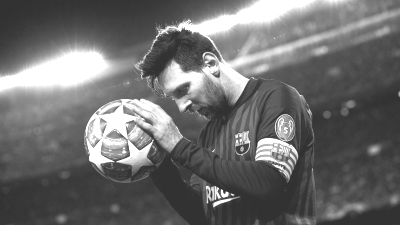
\includegraphics[width=5cm, height=5cm]{orgi/gMessi.jpg}
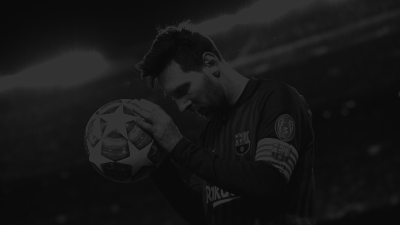
\includegraphics[width=5cm, height=5cm]{3_3/multi_constG1.jpg}
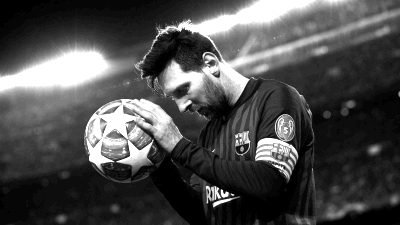
\includegraphics[width=5cm, height=5cm]{3_3/nmulti_constG1.jpg}
\caption{(Od lewej):obraz wejściowy, obraz po przemnożeniu przez liczbę=50,
obraz po normalizacji}
\end{figure}
\begin{figure}[h]
\centering
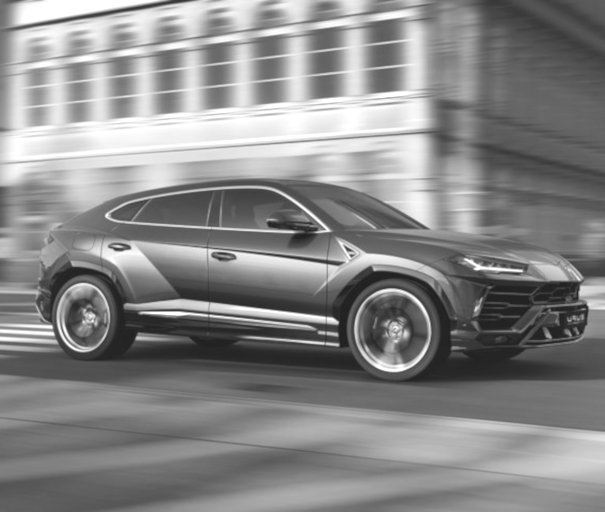
\includegraphics[width=5cm, height=5cm]{orgi/gLU.jpg}
\includegraphics[width=5cm, height=5cm]{3_3/multi_constG2.jpg}
\includegraphics[width=5cm, height=5cm]{3_3/nmulti_constG2.jpg}
\caption{(Od lewej): obraz wejściowy, obraz po przemnożeniu przez liczbę=100, obraz po normalizacji}
\end{figure}

\newpage
\textbf{\Large Kod funkcji}
   
\lstset{language=Python}
\vspace{0.25cm}
\begin{lstlisting}[caption={Mnożenie obrazu przez zadaną liczbę}]

def multiplication_const_grayscale(image1, const=1):

    fmax = 0
    fmin = 256

    if image1.imageBitsColor[0] == 4:

        maxBitsColor = 15
        if not (0 < const <= 15):
            raise Exception("program do obrazow SZARYCH 4 bitowych moze
             pomnozyc liczbe z zakresu 0-15, a podana liczba "
                            "to %d." % const)
    else:
        if image1.imageBitsColor[0] == 8:

            maxBitsColor = 255
            if not (0 < const <= 255):
                raise Exception("program do obrazow SZARYCH 8 bitowych
                 moze pomnozyc liczbe z zakresu 0-255, a podana "
                                "podana to %d." % const)
        else:
            raise Exception("program mnozy jedynie obrazy SZARE 4, 8 bitowe
             ze stala")

    # mnozenie
    for i in range(image1.imageLength):
        for j in range(image1.imageWidth):
            tempMult = image1.imageData[i][j][0]

            if tempMult == maxBitsColor:
                tempMult = const

            elif tempMult == 0:
                tempMult = 0

            else:
                tempMult = ceil((image1.imageData[i][j][0] * const) /
                 maxBitsColor)

            image1.imageData[i][j][0] = tempMult

            if tempMult > fmax:
                fmax = tempMult

            if tempMult < fmin:
                fmin = tempMult

    writeTiff('multi_const', image1)

    # normalizacja
    for i in range(image1.imageLength):
        for j in range(image1.imageWidth):
            image1.imageData[i][j][0] = round(maxBitsColor *
             ((image1.imageData[i][j][0] - fmin) / (fmax - fmin)))

    writeTiff('normalization_multi_const', image1)

\end{lstlisting}
\newpage


\section{Mnożenie obrazu przez inny obraz}

\vspace{0.5cm}\textbf{\Large Opis ćwiczenia}
\vspace{0.25cm}\newline
Algebraiczne mnożenie obrazów f i f’ jest określone jedynie dla obrazów o tych samych wymiarach M x N i strukturze ich macierzy i wykonuje się mnożąc każdy element obrazu P1 przez odpowiadający piksel drugiego obrazu P2.
\newline
\newline
\textbf{\Large Opis realizowanych operacji}
\begin{enumerate}
\item Weź dwa identycznych rozmiarów obrazy $P_1 i P_2$
\item Dla wszystkich pikseli w obrazie wykonaj:  
\item Jeśli składowa barwy piksla ma maksymalną głębię koloru to składowa wynikowa otrzymuje wartość odpowiadającą wartości składowej drugiego obrazu
\item W przeciwnym wypadku, jeśli składowa barwy pikslu ma wartość 0 to składowa wynikowa otrzymuje wartość 0
\item W przeciwnym wypadku mnóż odpowiednie sobie składowe, a wynik dziel przez maksymalną głębię koloru, zaokrąglając do najbliższej większej liczby całkowitej
\item Znormalizowanie obrazu wzorem:
\newline $f_{norm}=Z_{rep}[(f-f_{min})/(f_{max}-f_{min})]$
\end{enumerate}

\vspace{0.5cm}
\textbf{\Large Kod do wykonania danego problemu}
\lstset{language=Python}
\vspace{0.25cm}
\begin{lstlisting}
	nameFIleONE = 'img/gae.tif'
	nameFileTWO = 'img/gMessi.tif'
	readFileOne = ReadTiff(nameFIleONE)
	imageOne = Image(readFileOne)
	readFileTwo = ReadTiff(nameFileTWO)
	imageTwo = Image(readFileTwo)
	unification_Grayscale_Geometric(imageOne, imageTwo)
	unification_Grayscale_Resolution(imageOne, imageTwo) 
	multiplication_two_images_grayscale(imageOne, imageTwo)
	
	nameFIleTHREE = 'img/gLU.tif'
	nameFileFOUR = 'img/groza.tif'
	readFileThree = ReadTiff(nameFIleTHREE)
	imageThree = Image(readFileThree)
	readFileFour = ReadTiff(nameFileFOUR)
	imageFour = Image(readFileFour)
	unification_Grayscale_Geometric(imageThree, imageFour)
	unification_Grayscale_Resolution(imageThree, imageFour)
	multiplication_two_images_grayscale(imageThree, imageFour)

\end{lstlisting}


\newpage
\vspace{0.25cm}\textbf{\Large Przeprowadzone testy}
\vspace{0.5cm}
\begin{figure}[h]
\centering
\includegraphics[width=6cm, height=6cm]{2_2/ResolG1.jpg}
\includegraphics[width=6cm, height=6cm]{2_2/ResolG2.jpg}
\caption{Obrazy wejściowe (od lewej):pierwszy obraz wejściowy,drugi obraz wejściowy}
\end{figure}
\begin{figure}[h]
\centering
\includegraphics[width=6cm, height=6cm]{3_4/multi_twoG1.jpg}
\includegraphics[width=6cm, height=6cm]{3_4/nmulti_twoG1.jpg}
\caption{Obrazy wyjściowe (od lewej): obraz powstały w wyniku mnożenia dwóch obrazów, obraz wynikowy po normalizacji}
\end{figure}

\newpage
\begin{figure}[h]
\centering
\includegraphics[width=6cm, height=6cm]{2_2/ResolG3.jpg}
\includegraphics[width=6cm, height=6cm]{2_2/ResolG4.jpg}
\caption{Obrazy wejściowe (od lewej):pierwszy obraz wejściowy,drugi obraz wejściowy}
\end{figure}
\begin{figure}[h]
\centering
\includegraphics[width=6cm, height=6cm]{3_4/multi_twoG2.jpg}
\includegraphics[width=6cm, height=6cm]{3_4/nmulti_twoG2.jpg}
\caption{Obrazy wyjściowe (od lewej): obraz powstały w wyniku mnożenia dwóch obrazów, obraz wynikowy po normalizacji}
\end{figure}

\newpage
\textbf{\Large Kod funkcji}
   
\lstset{language=Python}
\vspace{0.25cm}
\begin{lstlisting}[caption={Mnożenie dwóch obrazów}]

def multiplication_two_images_grayscale(image1, image2):

    global maxBitsColor
    fmax = 0
    fmin = 256

    if image1.imageBitsColor[0] == image2.imageBitsColor[0] and
     (image1.imageLength == image2.imageLength) and
      (image1.imageWidth == image2.imageWidth):

        if image1.imageBitsColor[0] == 4:
            maxBitsColor = 15

        elif image1.imageBitsColor[0] == 8:
            maxBitsColor = 255

    else:
        raise Exception("program mnozy jedynie obrazy SZARE 4, 8 bitowe
         oraz obrazy musza miec takie same rozmiary.")

    # mnozenie
    for i in range(image1.imageLength):
        for j in range(image1.imageWidth):
            tempMult = image1.imageData[i][j][0]

            if tempMult == maxBitsColor:
                tempMult = image2.imageData[i][j][0]

            elif tempMult == 0:
                tempMult = 0

            else:
                tempMult = ceil((image1.imageData[i][j][0] *
                 image2.imageData[i][j][0]) / maxBitsColor)

            image1.imageData[i][j][0] = tempMult

            if tempMult > fmax:
                fmax = tempMult

            if tempMult < fmin:
                fmin = tempMult

    writeTiff('multi_two_images', image1)

    # normalizacja
    for i in range(image1.imageLength):
        for j in range(image1.imageWidth):
            image1.imageData[i][j][0] = round(maxBitsColor *
             ((image1.imageData[i][j][0] - fmin) / (fmax - fmin)))

    writeTiff('normalization_multi_two_images', image1)

\end{lstlisting}
\newpage

\section{Mieszanie obrazów z okreslonym współczynnikiem}

\vspace{0.5cm}\textbf{\Large Opis ćwiczenia}
\vspace{0.25cm}\newline
Mieszanie dwóch obrazów polega na sumowaniu ich z wagami $\alpha$ i $(1-\alpha)$, odpowiednio
\newline według wzoru: $f_m=f*\alpha+f'*(1-\alpha)$, gdzie $\alpha\in[0,1]$. Płynna zmiana parametru $\alpha$ w przedziale [0, 1] powoduje efekt przechodzenia obrazu f' w obraz f
\newline
\newline
\textbf{\Large Opis realizowanych operacji}
\begin{enumerate}
\item Weź dwa identycznych rozmiarów obrazy $P_1 i P_2$
\item Określ współczynnik mieszania $\alpha$ wyrażony jako liczba rzeczywista z zakresu < 0, 1 >; \newline 0 reprezentuje pewną przezroczystość, 1 - nieprzezroczystości
\item Dla wszystkich pikseli w obrazach wejściowych wykonuj: $Q(i,j)=\alpha*P_1(i,j)+(1-\alpha)*P_2(i,j)$
\end{enumerate}

\vspace{0.5cm}
\textbf{\Large Kod do wykonania danego problemu}
\lstset{language=Python}
\vspace{0.25cm}
\begin{lstlisting}
	nameFIleONE = 'img/gae.tif'
	nameFileTWO = 'img/gMessi.tif'
	readFileOne = ReadTiff(nameFIleONE)
	imageOne = Image(readFileOne)
	readFileTwo = ReadTiff(nameFileTWO)
	imageTwo = Image(readFileTwo)
	unification_Grayscale_Geometric(imageOne, imageTwo)
	unification_Grayscale_Resolution(imageOne, imageTwo) 
	mixing_images_grayscale(imageOne, imageTwo, 0.5)
	
	nameFIleTHREE = 'img/gLU.tif'
	nameFileFOUR = 'img/groza.tif'
	readFileThree = ReadTiff(nameFIleTHREE)
	imageThree = Image(readFileThree)
	readFileFour = ReadTiff(nameFileFOUR)
	imageFour = Image(readFileFour)
	unification_Grayscale_Geometric(imageThree, imageFour)
	unification_Grayscale_Resolution(imageThree, imageFour)
	mixing_images_grayscale(imageThree, imageFour, 0.8)

\end{lstlisting}


\newpage
\vspace{0.25cm}\textbf{\Large Przeprowadzone testy}
\vspace{0.5cm}
\begin{figure}[h]
\centering
\includegraphics[width=6cm, height=6cm]{2_2/ResolG1.jpg}
\includegraphics[width=6cm, height=6cm]{2_2/ResolG2.jpg}
\caption{Obrazy wejściowe (od lewej):pierwszy obraz wejściowy,drugi obraz wejściowy}
\end{figure}
\begin{figure}[h]
\centering
\includegraphics[width=6cm, height=6cm]{3_5/mixG1.jpg}
%\includegraphics[width=6cm, height=6cm]{3_5/nmixG1.jpg}
\caption{Obrazy wyjściowe (od lewej): obraz powstały w wyniku
mieszania obrazów ze współczynnikiem $\alpha=0.5$}
\end{figure}

\newpage
\begin{figure}[h]
\centering
\includegraphics[width=6cm, height=6cm]{2_2/ResolG3.jpg}
\includegraphics[width=6cm, height=6cm]{2_2/ResolG4.jpg}
\caption{Obrazy wejściowe (od lewej):pierwszy obraz wejściowy,drugi obraz wejściowy}
\end{figure}
\begin{figure}[h]
\centering
\includegraphics[width=6cm, height=6cm]{3_5/mixG2.jpg}
%\includegraphics[width=6cm, height=6cm]{3_5/nmixG2.jpg}
\caption{Obrazy wyjściowe (od lewej): obraz powstały w wyniku
mieszania obrazów ze współczynnikiem $\alpha=0.8$}
\end{figure}

\newpage
\textbf{\Large Kod funkcji}
   
\lstset{language=Python}
\vspace{0.25cm}
\begin{lstlisting}[caption={Mieszanie obrazów z okreslonym współczynnikiem}]

def mixing_images_grayscale(image1, image2, scales=0.0):

    global maxBitsColor
    fmax = 0
    fmin = 256

    if image1.imageBitsColor[0] == image2.imageBitsColor[0] and
     (image1.imageLength == image2.imageLength) and
      (image1.imageWidth == image2.imageWidth):

        if not (0.0 <= scales <= 1.0):
            raise Exception("program miesza obrazy SZARE z waga
             z zakresu 0.0-1.0, a podana liczba to %f." %scales)

        if image1.imageBitsColor[0] == 4:
            maxBitsColor = 15

        elif image1.imageBitsColor[0] == 8:
            maxBitsColor = 255

    else:
        raise Exception("program miesza jedynie obrazy SZARE 4, 8 bitowe 
        oraz obrazy musza miec takie same rozmiary.")

    for i in range(image1.imageLength):
        for j in range(image1.imageWidth):
            tempMix = ceil(scales * image1.imageData[i][j][0] +
            (1 - scales) * image2.imageData[i][j][0])
            image1.imageData[i][j][0] = tempMix

            if tempMix > fmax:
                fmax = tempMix

            if tempMix < fmin:
                fmin = tempMix

    writeTiff('mix_two_image', image1)
        
\end{lstlisting}
\newpage


\section{Potęgowanie obrazu (z zadaną potęgą)}

\vspace{0.5cm}\textbf{\Large Opis ćwiczenia}
\vspace{0.25cm}\newline
Potęgowanie obrazu jest szczególnym przypadkiem operacji mnożenia obrazów.
\newline
\newline

\vspace{0.5cm}
\textbf{\Large Kod do wykonania danego problemu}
\lstset{language=Python}
\vspace{0.25cm}
\begin{lstlisting}
	nameFileTWO = 'img/gMessi.tif'
	readFileTwo = ReadTiff(nameFileTWO)
	imageTwo = Image(readFileTwo)

	pow_image_grayscale(imageTwo, 2)
	
	nameFIleTHREE = 'img/gLU.tif'
	readFileThree = ReadTiff(nameFIleTHREE)
	imageThree = Image(readFileThree)
	
	pow_image_grayscale(imageThree, 3)

\end{lstlisting}

\vspace{0.25cm}\textbf{\Large Przeprowadzone testy}
\vspace{0.5cm}
\begin{figure}[h]
\centering
\includegraphics[width=5cm, height=5cm]{orgi/gMessi.jpg}
\includegraphics[width=5cm, height=5cm]{3_6/powG1.jpg}
\includegraphics[width=5cm, height=5cm]{3_6/npowG1.jpg}
\caption{(Od lewej):obraz wejściowy, obraz po podniesieniu do potęgi $\alpha=2$,
obraz po normalizacji}
\end{figure}
\begin{figure}[h]
\centering
\includegraphics[width=5cm, height=5cm]{orgi/gLU.jpg}
\includegraphics[width=5cm, height=5cm]{3_6/powG2.jpg}
\includegraphics[width=5cm, height=5cm]{3_6/npowG2.jpg}
\caption{(Od lewej):obraz wejściowy, obraz po podniesieniu do potęgi $\alpha=3$,
obraz po normalizacji}
\end{figure}

\newpage
\textbf{\Large Kod funkcji}
   
\lstset{language=Python}
\vspace{0.25cm}
\begin{lstlisting}[caption={Potęgowanie obrazu}]

def pow_image_grayscale(image1, p=1):

    global maxBitsColor
    fmax = 0
    fmin = 256
    fmaximage = 0

    if not (0 < p):
        raise Exception("program poteguje obraz SZARY z zadana potega 
        z zakresu p > 0, a podana liczba "
                        "to %d." % p)

    if image1.imageBitsColor[0] == 4:
        maxBitsColor = 15
    elif image1.imageBitsColor[0] == 8:
        maxBitsColor = 255

    for i in range(image1.imageLength):
        for j in range(image1.imageWidth):
            tempPow = image1.imageData[i][j][0]
            if tempPow > fmaximage:
                fmaximage = tempPow

    for i in range(image1.imageLength):
        for j in range(image1.imageWidth):
            tempPow = image1.imageData[i][j][0]

            if tempPow == maxBitsColor:
                tempPow = maxBitsColor
            elif tempPow == 0:
                tempPow = 0
            else:
                tempPow = pow(image1.imageData[i][j][0] / fmaximage, p) *
                 maxBitsColor

            image1.imageData[i][j][0] = ceil(tempPow)

            if tempPow > fmax:
                fmax = tempPow

            if tempPow < fmin:
                fmin = tempPow

    writeTiff('pow_image', image1)
    # normalizacja
    for i in range(image1.imageLength):
        for j in range(image1.imageWidth):
            image1.imageData[i][j][0] = round(maxBitsColor * 
            ((image1.imageData[i][j][0] - fmin) / (fmax - fmin)))

    writeTiff('normalization_pow_image', image1)

\end{lstlisting}


\newpage
\section{Dzielenie obrazu przez (zadaną) liczbę}

\textbf{\Large Opis realizowanych operacji}
\begin{enumerate}
\item Dla wszystkich piksli w tym obrazie wykonaj:
\item Policz sumę piksli ze stałą
\item Wybierz największą sumę $Q_{max}$ i policz równania $Q[i,j]=(S*$maksymalna głębia koloru$)/Q_{max}$. Wynik zaokrąglij do najbliższej górnej liczby całkowitej
\item Znormalizowanie obrazu wzorem:
\newline $f_{norm}=Z_{rep}[(f-f_{min})/(f_{max}-f_{min})]$
\end{enumerate}

\vspace{0.5cm}
\textbf{\Large Kod do wykonania danego problemu}
\lstset{language=Python}
\vspace{0.25cm}
\begin{lstlisting}
	nameFileTWO = 'img/gMessi.tif'
	readFileTwo = ReadTiff(nameFileTWO)
	imageTwo = Image(readFileTwo)
	division_const_grayscale(imageTwo, 15)
	
	nameFIleTHREE = 'img/gLU.tif'
	readFileThree = ReadTiff(nameFIleTHREE)
	imageThree = Image(readFileThree)
	division_const_grayscale(imageThree, 3)

\end{lstlisting}


\vspace{0.25cm}\textbf{\Large Przeprowadzone testy}
\vspace{0.5cm}

\begin{figure}[h]
\centering
\includegraphics[width=5cm, height=5cm]{orgi/gMessi.jpg}
\includegraphics[width=5cm, height=5cm]{3_7/div_constG1.jpg}
\includegraphics[width=5cm, height=5cm]{3_7/ndiv_constG1.jpg}
\caption{(Od lewej):obraz wejściowy,  obraz po podzieleniu przez liczbę=15,
obraz po normalizacji}
\end{figure}
\begin{figure}[h]
\centering
\includegraphics[width=5cm, height=5cm]{orgi/gLU.jpg}
\includegraphics[width=5cm, height=5cm]{3_7/div_constG2.jpg}
\includegraphics[width=5cm, height=5cm]{3_7/ndiv_constG2.jpg}
\caption{(Od lewej):obraz wejściowy, obraz po podzieleniu przez liczbę=3,
obraz po normalizacji}
\end{figure}

\newpage
\textbf{\Large Kod funkcji}
   
\lstset{language=Python}
\vspace{0.25cm}
\begin{lstlisting}[caption={Dzielnie obrazu przez liczbę}]

def division_const_grayscale(image1, const=1):

    Qmax = 0
    fmax = 0
    fmin = 256

    if image1.imageBitsColor[0] == 4:

        maxBitsColor = 15
        if not (0 < const <= 15):
            raise Exception("program do obrazow SZARYCH 4 bitowych 
            moze dzielic liczbe z zakresu 0-15, a podana liczba "
                            "to %d." % const)
    elif image1.imageBitsColor[0] == 8:

        maxBitsColor = 255
        if not (0 < const <= 255):
            raise Exception("program do obrazow SZARYCH 8 bitowych
            moze dzielic liczbe z zakresu 0-255, a podana "
                            "podana to %d." % const)
    else:
        raise Exception("program dzieli jedynie obrazy SZARE 4, 8 bitowe 
        ze stala")

    for i in range(image1.imageLength):
        for j in range(image1.imageWidth):
            tempDiv = image1.imageData[i][j][0] + const

            if Qmax < tempDiv:
                Qmax = tempDiv

    for i in range(image1.imageLength):
        for j in range(image1.imageWidth):
            tempDiv = image1.imageData[i][j][0] + const

            resultDiv = (tempDiv * maxBitsColor) / Qmax

            image1.imageData[i][j][0] = ceil(resultDiv)

            if resultDiv > fmax:
                fmax = resultDiv

            if resultDiv < fmin:
                fmin = resultDiv

    writeTiff('div_image_const', image1)
    # normalizacja
    for i in range(image1.imageLength):
        for j in range(image1.imageWidth):
            image1.imageData[i][j][0] = round(maxBitsColor * 
            ((image1.imageData[i][j][0] - fmin) / (fmax - fmin)))

    writeTiff('normalization_div_image_const', image1)

\end{lstlisting}
\newpage



\section{Dzielenie obrazu przez inny obraz}

\textbf{\Large Opis realizowanych operacji}
\begin{enumerate}
\item Weź dwa identycznych rozmiarów obrazy $P_1 i P_2$
\item Dla wszystkich pikseli w obrazie wykonaj:  
\item Policz sumy pikseli ze stałą
\item Wybierz największą sumę $Q_{max}$ i policz równanie:
\newline $Q[i,j]=(S-$maksymalna głębia koloru$)/Q_{max}$
\newline Wynik zaokrąglij do najbliższej górnej liczby całkowitej.
\item Znormalizowanie obrazu wzorem:
\newline $f_{norm}=Z_{rep}[(f-f_{min})/(f_{max}-f_{min})]$
\end{enumerate}

\vspace{0.5cm}
\textbf{\Large Kod do wykonania danego problemu}
\lstset{language=Python}
\vspace{0.25cm}
\begin{lstlisting}
	nameFIleONE = 'img/gae.tif'
	nameFileTWO = 'img/gMessi.tif'
	readFileOne = ReadTiff(nameFIleONE)
	imageOne = Image(readFileOne)
	readFileTwo = ReadTiff(nameFileTWO)
	imageTwo = Image(readFileTwo)
	unification_Grayscale_Geometric(imageOne, imageTwo)
	unification_Grayscale_Resolution(imageOne, imageTwo) 
	division_two_iamges_grayscale(imageOne, imageTwo)
	
	nameFIleTHREE = 'img/gLU.tif'
	nameFileFOUR = 'img/groza.tif'
	readFileThree = ReadTiff(nameFIleTHREE)
	imageThree = Image(readFileThree)
	readFileFour = ReadTiff(nameFileFOUR)
	imageFour = Image(readFileFour)
	unification_Grayscale_Geometric(imageThree, imageFour)
	unification_Grayscale_Resolution(imageThree, imageFour)
	division_two_iamges_grayscale(imageThree, imageFour)

\end{lstlisting}



\newpage
\vspace{0.25cm}\textbf{\Large Przeprowadzone testy}
\vspace{0.5cm}
\begin{figure}[h]
\centering
\includegraphics[width=6cm, height=6cm]{2_2/ResolG1.jpg}
\includegraphics[width=6cm, height=6cm]{2_2/ResolG2.jpg}
\caption{Obrazy wejściowe (od lewej):pierwszy obraz wejściowy,drugi obraz wejściowy}
\end{figure}
\begin{figure}[h]
\centering
\includegraphics[width=6cm, height=6cm]{3_8/div_twoG1.jpg}
\includegraphics[width=6cm, height=6cm]{3_8/ndiv_twoG1.jpg}
\caption{Obrazy wyjściowe (od lewej): obraz powstały w wyniku
podzielenia obrazów, obraz wynikowy po normalizacji}
\end{figure}

\newpage
\begin{figure}[h]
\centering
\includegraphics[width=6cm, height=6cm]{2_2/ResolG3.jpg}
\includegraphics[width=6cm, height=6cm]{2_2/ResolG4.jpg}
\caption{Obrazy wejściowe (od lewej):pierwszy obraz wejściowy,drugi obraz wejściowy}
\end{figure}
\begin{figure}[h]
\centering
\includegraphics[width=6cm, height=6cm]{3_8/div_twoG2.jpg}
\includegraphics[width=6cm, height=6cm]{3_8/ndiv_twoG2.jpg}
\caption{Obrazy wyjściowe (od lewej): obraz powstały w wyniku
podzielenia obrazów, obraz wynikowy po normalizacji}
\end{figure}

\newpage
\textbf{\Large Kod funkcji}
   
\lstset{language=Python}
\vspace{0.25cm}
\begin{lstlisting}[caption={Dzielenie dwóch obrazów}]

def division_two_iamges_grayscale(image1, image2):

    global maxBitsColor
    fmax = 0
    fmin = 256
    Qmax = 0

    if image1.imageBitsColor[0] == image2.imageBitsColor[0] and
    (image1.imageLength == image2.imageLength) and
     (image1.imageWidth == image2.imageWidth):

        if image1.imageBitsColor[0] == 4:
            maxBitsColor = 15

        elif image1.imageBitsColor[0] == 8:
            maxBitsColor = 255

    else:
        raise Exception("program dzieli jedynie obrazy SZARE 4, 8 bitowe
         oraz obrazy musza miec takie same rozmiary.")

    for i in range(image1.imageLength):
        for j in range(image1.imageWidth):
            tempDiv = image1.imageData[i][j][0] + image2.imageData[i][j][0]

            if Qmax < tempDiv:
                Qmax = tempDiv

    for i in range(image1.imageLength):
        for j in range(image1.imageWidth):
            tempDiv = image1.imageData[i][j][0] + image2.imageData[i][j][0]

            resultDiv = (tempDiv * maxBitsColor) / Qmax

            image1.imageData[i][j][0] = ceil(resultDiv)

            if resultDiv > fmax:
                fmax = resultDiv

            if resultDiv < fmin:
                fmin = resultDiv

    writeTiff('div_two_images', image1)
    # normalizacja
    for i in range(image1.imageLength):
        for j in range(image1.imageWidth):
            image1.imageData[i][j][0] = round(maxBitsColor *
             ((image1.imageData[i][j][0] - fmin) / (fmax - fmin)))

    writeTiff('normalization_div_two_images', image1)

\end{lstlisting}


\newpage
\section{Pierwiastkowanie obrazu}

\vspace{0.5cm}\textbf{\Large Opis ćwiczenia}
\vspace{0.25cm}\newline
Pierwiastkowanie obrazu jest szczególnym przypadkiem operacji potęgowania obrazów,
gdzie wykładnikiem jest ułamek.
\newline
\newline

\vspace{0.5cm}
\textbf{\Large Kod do wykonania danego problemu}
\lstset{language=Python}
\vspace{0.25cm}
\begin{lstlisting}
	nameFileTWO = 'img/gMessi.tif'
	readFileTwo = ReadTiff(nameFileTWO)
	imageTwo = Image(readFileTwo)
	sqrt_image_grayscale(imageTwo, 2)
	
	nameFIleTHREE = 'img/gLU.tif'
	readFileThree = ReadTiff(nameFIleTHREE)
	imageThree = Image(readFileThree)
	sqrt_image_grayscale(imageThree, 3)

\end{lstlisting}
\newpage


\vspace{0.25cm}\textbf{\Large Przeprowadzone testy}
\vspace{0.5cm}
\begin{figure}[h]
\centering
\includegraphics[width=5cm, height=5cm]{orgi/gMessi.jpg}
\includegraphics[width=5cm, height=5cm]{3_9/rootG1.jpg}
\includegraphics[width=5cm, height=5cm]{3_9/nrootG1.jpg}
\caption{(Od lewej):obraz wejściowy, obraz po spierwiastkowaniu pierwiastkiem kwadratowym, obraz po normalizacji}
\end{figure}
\begin{figure}[h]
\centering
\includegraphics[width=5cm, height=5cm]{orgi/gLU.jpg}
\includegraphics[width=5cm, height=5cm]{3_9/rootG2.jpg}
\includegraphics[width=5cm, height=5cm]{3_9/nrootG2.jpg}
\caption{(Od lewej): obraz wejściowy, obraz po spierwiastkowaniu pierwiastkiem stopnia trzeciego, obraz po normalizacji}
\end{figure}

\newpage
\textbf{\Large Kod funkcji}
   
\lstset{language=Python}
\vspace{0.25cm}
\begin{lstlisting}[caption={Pierwiastkowanie obrazu}]

def sqrt_image_grayscale(image1, deg=1):

    global maxBitsColor
    fmax = 0
    fmin = 256
    fmaximage = 0

    p = 1/deg

    if image1.imageBitsColor[0] == 4:
        maxBitsColor = 15
    elif image1.imageBitsColor[0] == 8:
        maxBitsColor = 255

    for i in range(image1.imageLength):
        for j in range(image1.imageWidth):
            tempPow = image1.imageData[i][j][0]
            if tempPow > fmaximage:
                fmaximage = tempPow

    for i in range(image1.imageLength):
        for j in range(image1.imageWidth):
            tempPow = image1.imageData[i][j][0]

            if tempPow == maxBitsColor:
                tempPow = maxBitsColor
            elif tempPow == 0:
                tempPow = 0
            else:
                tempPow = pow(image1.imageData[i][j][0] / fmaximage, p) *
                 maxBitsColor

            image1.imageData[i][j][0] = ceil(tempPow)

            if tempPow > fmax:
                fmax = tempPow

            if tempPow < fmin:
                fmin = tempPow

    writeTiff('root_image', image1)
    # normalizacja
    for i in range(image1.imageLength):
        for j in range(image1.imageWidth):
            image1.imageData[i][j][0] = round(maxBitsColor * 
            ((image1.imageData[i][j][0] - fmin) / (fmax - fmin)))

    writeTiff('normalization_root_image', image1)

\end{lstlisting}
\newpage


\section{Logarytmowanie obrazu}

\vspace{0.5cm}\textbf{\Large Opis ćwiczenia}
\vspace{0.25cm}\newline
Przesunięcie funkcji obrazowej f do góry o 1 przed jej logarytmowaniem wynika z
nieokreśloności logarytmu w zerze. Logarytmowanie obrazu powoduje rozjaśnienie i zróżnicowanie najciemniejszych obszarów obrazu.
\newline
\newline

\vspace{0.5cm}
\textbf{\Large Kod do wykonania danego problemu}
\lstset{language=Python}
\vspace{0.25cm}
\begin{lstlisting}
	nameFileTWO = 'img/gMessi.tif'
	readFileTwo = ReadTiff(nameFileTWO)
	imageTwo = Image(readFileTwo)
	log_image_grayscale(imageTwo)
	
	nameFIleTHREE = 'img/gLU.tif'
	readFileThree = ReadTiff(nameFIleTHREE)
	imageThree = Image(readFileThree)
	log_image_grayscale(imageThree)

\end{lstlisting}
\newpage

\vspace{0.25cm}\textbf{\Large Przeprowadzone testy}
\vspace{0.5cm}
\begin{figure}[h]
\centering
\includegraphics[width=5cm, height=5cm]{orgi/gMessi.jpg}
\includegraphics[width=5cm, height=5cm]{3_10/logG1.jpg}
\includegraphics[width=5cm, height=5cm]{3_10/nlogG1.jpg}
\caption{(Od lewej):obraz wejściowy, obraz po logarytmowaniu logarytmem
naturalnym, obraz po normalizacji}
\end{figure}
\begin{figure}[h]
\centering
\includegraphics[width=5cm, height=5cm]{orgi/gLU.jpg}
\includegraphics[width=5cm, height=5cm]{3_10/logG2.jpg}
\includegraphics[width=5cm, height=5cm]{3_10/nlogG2.jpg}
\caption{(Od lewej): obraz wejściowy, obraz po logarytmowaniu logarytmem
naturalnym, obraz po normalizacji}
\end{figure}

\newpage
\textbf{\Large Kod funkcji}
   
\lstset{language=Python}
\vspace{0.25cm}
\begin{lstlisting}[caption={Logarytmowanie obrazu}]

def log_image_grayscale(image1):

    global maxBitsColor
    fmax = 0
    fmin = 256
    fmaximage = 0

    if image1.imageBitsColor[0] == 4:
        maxBitsColor = 15
    elif image1.imageBitsColor[0] == 8:
        maxBitsColor = 255

    for i in range(image1.imageLength):
        for j in range(image1.imageWidth):
            tempLog = image1.imageData[i][j][0]
            if fmaximage < tempLog:
                fmaximage = tempLog

    for i in range(image1.imageLength):
        for j in range(image1.imageWidth):
            tempLog = image1.imageData[i][j][0]

            if tempLog == 0:
                tempLog = 0
            else:
                tempLog = (log(1 + tempLog) / log(1+fmaximage))*maxBitsColor

            image1.imageData[i][j][0] = ceil(tempLog)

            if tempLog > fmax:
                fmax = tempLog

            if tempLog < fmin:
                fmin = tempLog

    writeTiff('log_image', image1)
    # normalizacja
    for i in range(image1.imageLength):
        for j in range(image1.imageWidth):
            image1.imageData[i][j][0] = round(maxBitsColor * 
            ((image1.imageData[i][j][0] - fmin) / (fmax - fmin)))

    writeTiff('normalization_log_image', image1)

\end{lstlisting}




\chapter{Operacje sumowania arytmetycznego obrazów barwowychh}
\section{Sumowanie (okreslonej) stałej z obrazem}

\vspace{0.5cm}\textbf{\Large Opis ćwiczenia}
\vspace{0.25cm}\newline
Algorytm sumowania obrazu barwowego z określoną stałą polega na dodaniu do każdej
wartości
pojedynczego piksla stałej liczby. Po operacji sumowania następuje normalizacja
obrazu.
\newline
\newline
\textbf{\Large Opis realizowanych operacji}
\begin{enumerate}
\item Policz sumy wartości każdego piksla ze stałą.
\item Jeśli przynajmniej jedna z tych sum jest większa od głębi kolorów obrazu to:
\item Wybierz największą sumę $Q_{max}$ i $D_{max}$ policz ze wzoru
\newline $D_{max}[i,j]=(Q_{max}[i,j]$ - głębia koloru obrazu$)$
\item Policz proporcję $X=D_{max}[i,j]/$głębia koloru obrazu 
\newline i zaokrąglając wynik do najbliższej z góry liczby całkowitej.
\item Jeśli nie ma sumy większej od głębi kolorów obrazu to X=0.
\item Policz sumy: 
\newline $Q_R[i,j]=P_R[i,j]-(P_R[i,j]*X)+const-(const*X)$
\newline $Q_G[i,j]=P_G[i,j]-(P_G[i,j]*X)+const-(const*X)$
\newline $Q_B[i,j]=P_B[i,j]-(P_B[i,j]*X)+const-(const*X)$
\item Znormalizowanie obrazu wzorem:
\newline $f_{norm}=Z_{rep}[(f-f_{min})/(f_{max}-f_{min})]$
\end{enumerate}

\newpage
\vspace{0.5cm}
\textbf{\Large Kod do wykonania danego problemu}
\lstset{language=Python}
\vspace{0.25cm}
\begin{lstlisting}

	nameFIleONE = 'img/RGBMessi.tif'
	readFileOne = ReadTiff(nameFIleONE)
	imageOne = Image(readFileOne)
	sum_const_RGB(imageOne, 50)
	
	nameFileFOUR = 'img/RGBkulki.tif'
	readFileFour = ReadTiff(nameFileFOUR)
	imageFour = Image(readFileFour)
	sum_const_RGB(imageFour, 100)

\end{lstlisting}

%\newpage
\vspace{0.25cm}\textbf{\Large Przeprowadzone testy}
\vspace{0.5cm}
\begin{figure}[h]
\centering
\includegraphics[width=5cm, height=5cm]{orgi/RGBMessi.jpg}
\includegraphics[width=5cm, height=5cm]{4_1/addconstRGB1.jpg}
\includegraphics[width=5cm, height=5cm]{4_1/naddconstRGB1.jpg}
\caption{(Od lewej): obraz wejściowy RGB, obraz po sumowaniu ze stałą = 50, obraz po normalizacji}
\end{figure}
\begin{figure}[h]
\centering
\includegraphics[width=5cm, height=5cm]{orgi/RGBkulki.jpg}
\includegraphics[width=5cm, height=5cm]{4_1/addconstRGB2.jpg}
\includegraphics[width=5cm, height=5cm]{4_1/naddconstRGB2.jpg}
\caption{(Od lewej): obraz wejściowy RGB, obraz po sumowaniu ze stałą = 100, obraz po normalizacji}
\end{figure}

\newpage
\textbf{\Large Kod funkcji}
   
\lstset{language=Python}
\vspace{0.25cm}
\begin{lstlisting}[caption={Sumowanie (okreslonej) stałej z obrazem RGB}]

def sum_const_RGB(image1, const=0):

    if image1.imageBitsColor[0] == 4:

        maxBitsColor = 15
        if not (0 <= const <= 15):
            raise Exception("program do obrazow RGB 4 bitowych
             mozne dodac liczbe z zakresu 0-15, a podana liczba "
                            "to %d." % const)
    else:
        if image1.imageBitsColor[0] == 8:

            maxBitsColor = 255
            if not (0 <= const <= 255):
                raise Exception("program do obrazow RGB 8 bitowych
                 mozne dodac liczbe z zakresu 0-255, a podana "
                                "podana to %d." % const)
        else:
            raise Exception("program dodaje jedynie obrazy RGB 4, 8
             bitowe ze stala")

    Qmax = 0
    Dmax = 0
    X = 0
    fmax = 0
    fmin = 256

    for i in range(image1.imageLength):
        for j in range(image1.imageWidth):
            tempR = image1.imageData[i][j][0] + const
            tempG = image1.imageData[i][j][1] + const
            tempB = image1.imageData[i][j][2] + const

            if max([tempR, tempG, tempB]) > Qmax:
                Qmax = max([tempR, tempG, tempB])

    if Qmax > maxBitsColor:
        Dmax = Qmax - maxBitsColor
        X = round(Dmax/maxBitsColor, 2)

    if X == 1.0:
        X = 0.99

    print(X)
    # dodawanie
    for i in range(image1.imageLength):
        for j in range(image1.imageWidth):
            tempSumR = ceil((image1.imageData[i][j][0] -
             (image1.imageData[i][j][0] * X)) + (const - (const * X)))
            tempSumG = ceil((image1.imageData[i][j][1] -
             (image1.imageData[i][j][1] * X)) + (const - (const * X)))
            tempSumB = ceil((image1.imageData[i][j][2] -
             (image1.imageData[i][j][2] * X)) + (const - (const * X)))

            image1.imageData[i][j][0] = tempSumR
            image1.imageData[i][j][1] = tempSumG
            image1.imageData[i][j][2] = tempSumB

            if max([tempSumR, tempSumG, tempSumB]) > fmax:
                fmax = max([tempSumR, tempSumG, tempSumB])

            if min([tempSumR, tempSumG, tempSumB]) < fmin:
                fmin = min([tempSumR, tempSumG, tempSumB])

    writeTiff('add_const_RGB', image1)

    # normalizacja
    for i in range(image1.imageLength):
        for j in range(image1.imageWidth):
            image1.imageData[i][j][0] = ceil(maxBitsColor *
             ((image1.imageData[i][j][0] - fmin) / (fmax - fmin)))
            image1.imageData[i][j][1] = ceil(maxBitsColor *
             ((image1.imageData[i][j][1] - fmin) / (fmax - fmin)))
            image1.imageData[i][j][2] = ceil(maxBitsColor *
             ((image1.imageData[i][j][2] - fmin) / (fmax - fmin)))
    writeTiff('normalization_add_const_RGB', image1)


\end{lstlisting}


\newpage
\section{Sumowanie dwóch obrazów}

\vspace{0.5cm}\textbf{\Large Opis ćwiczenia}
\vspace{0.25cm}\newline
Algebraiczne sumowanie obrazów f i f’ jest określone jedynie dla obrazów o tych samych wymiarach M x N i strukturze ich macierzy. Algorytm sumowania obrazu z obrazem polega na dodaniu do wartości piksla z pierwszego obrazu, wartości odpowiadającego piksla z drugiego obrazu. Po operacji sumowania następuje normalizacja obrazu. Dodawanie obrazów jest użyteczne w uśrednianiu obrazów, wykonywanym w celu zredukowania na nich szumu.
\newline
\newline
\textbf{\Large Opis realizowanych operacji}
\begin{enumerate}
\item Weź dwa identycznych rozmiarów obrazy.
\item Dla wszystkich pikseli w tych obrazach wykonaj:
\item Policz sumy dla wszystkich piksli, odpowiadających składowych barw.
\item Jeśli przynajmniej jedna z tych sum jest większa od maksymalnej głębi kolorów obrazu to:
\item Wybierz największą sumę $Q_{max}$ i $D_{max}$ policz ze wzoru
\newline $D_{max}[i,j]=(Q_{max}[i,j]$ - głębia koloru obrazu$)$
\item Policz proporcję $X=D_{max}[i,j]/$głębia koloru obrazu 
\newline i zaokrąglając wynik do najbliższej z góry liczby całkowitej.
\item Jeśli nie ma sumy większej od głębi kolorów obrazu to X=0.
\item Policz sumy: 
\newline $Q_R[i,j]=P1_R[i,j]-(P1_R[i,j]*X)+P2_R[i,j]-(P2_R[i,j]*X)$
$Q_G[i,j]=P1_G[i,j]-(P1_G[i,j]*X)+P2_G[i,j]-(P2_G[i,j]*X)$
$Q_B[i,j]=P1_B[i,j]-(P1_B[i,j]*X)+P2_B[i,j]-(P2_B[i,j]*X)$
\item Znormalizowanie obrazu wzorem:
\newline $f_{norm}=Z_{rep}[(f-f_{min})/(f_{max}-f_{min})]$
\end{enumerate}

\newpage
\vspace{0.5cm}
\textbf{\Large Kod do wykonania danego problemu}
\lstset{language=Python}
\vspace{0.25cm}
\begin{lstlisting}
	nameFIleONE = 'img/RGBMessi.tif'
	nameFileTWO = 'img/RGBLL.tif'
	readFileOne = ReadTiff(nameFIleONE)
	imageOne = Image(readFileOne)
	readFileTwo = ReadTiff(nameFileTWO)
	imageTwo = Image(readFileTwo)
	unification_RGB_Geometric(imageOne, imageTwo)
	unification_RGB_Resolution(imageOne, imageTwo)
	sum_two_images_RGB(imageOne, imageTwo)
	
	nameFIleTHREE = 'img/RGBkamel.tif'
	nameFileFOUR = 'img/RGBkulki.tif'
	readFileThree = ReadTiff(nameFIleTHREE)
	imageThree = Image(readFileThree
	readFileFour = ReadTiff(nameFileFOUR)
	imageFour = Image(readFileFour)
	unification_RGB_Geometric(imageThree, imageFour)
	unification_RGB_Resolution(imageThree, imageFour)
	sum_two_images_RGB(imageThree, imageFour)

\end{lstlisting}


\newpage
\vspace{0.25cm}\textbf{\Large Przeprowadzone testy}
\vspace{0.5cm}
\begin{figure}[h]
\centering
\includegraphics[width=6cm, height=6cm]{2_4/ResolRGB1.jpg}
\includegraphics[width=6cm, height=6cm]{2_4/ResolRGB2.jpg}
\caption{Obrazy wejściowe (od lewej):pierwszy obraz wejściowy,drugi obraz wejściowy}
\end{figure}
\begin{figure}[h]
\centering
\includegraphics[width=6cm, height=6cm]{4_2/add_twoRGB1.jpg}
\includegraphics[width=6cm, height=6cm]{4_2/nadd_twoRGB1.jpg}
\caption{Obrazy wyjściowe (od lewej): obraz powstały w wyniku sumowania dwóch obrazów, obraz wynikowy po normalizacji}
\end{figure}

\newpage
\begin{figure}[h]
\centering
\includegraphics[width=6cm, height=6cm]{2_4/ResolRGB3.jpg}
\includegraphics[width=6cm, height=6cm]{2_4/ResolRGB4.jpg}
\caption{Obrazy wejściowe (od lewej):pierwszy obraz wejściowy,drugi obraz wejściowy}
\end{figure}
\begin{figure}[h]
\centering
\includegraphics[width=6cm, height=6cm]{4_2/add_twoRGB2.jpg}
\includegraphics[width=6cm, height=6cm]{4_2/nadd_twoRGB2.jpg}
\caption{Obrazy wyjściowe (od lewej): obraz powstały w wyniku sumowania dwóch obrazów, obraz wynikowy po normalizacji}
\end{figure}

\newpage
\textbf{\Large Kod funkcji}
   
\lstset{language=Python}
\vspace{0.25cm}
\begin{lstlisting}[caption={Sumowanie dwóch obrazów barwowych}]

def sum_two_images_RGB(image1, image2):

    global maxBitsColor
    if image1.imageBitsColor[0] == image2.imageBitsColor[0] and
     (image1.imageLength == image2.imageLength) and
      (image1.imageWidth == image2.imageWidth):

        if image1.imageBitsColor[0] == 4:
            maxBitsColor = 15

        else:
            if image1.imageBitsColor[0] == 8:
                maxBitsColor = 255

    else:
        raise Exception("program dodaje jedynie obrazy RGB 4, 8 bitowe
         oraz obrazy musza miec takie same rozmiary.")

    Qmax = 0
    Dmax = 0
    X = 0
    fmax = 0
    fmin = 256

    for i in range(image1.imageLength):
        for j in range(image1.imageWidth):
            tempR = image1.imageData[i][j][0] + image2.imageData[i][j][0]
            tempG = image1.imageData[i][j][1] + image2.imageData[i][j][1]
            tempB = image1.imageData[i][j][2] + image2.imageData[i][j][2]

            if max([tempR, tempG, tempB]) > Qmax:
                Qmax = max([tempR, tempG, tempB])

    if Qmax > maxBitsColor:
        Dmax = Qmax - maxBitsColor
        X = round(Dmax/maxBitsColor, 2)

    if X == 1.0:
        X = 0.99

    for i in range(image1.imageLength):
        for j in range(image1.imageWidth):
            tempSumR = ceil((image1.imageData[i][j][0] - 
            (image1.imageData[i][j][0] * X)) + 
            (image2.imageData[i][j][0] - (image2.imageData[i][j][0] * X)))

            image1.imageData[i][j][0] = tempSumR

            tempSumG = ceil((image1.imageData[i][j][1] - 
            (image1.imageData[i][j][1] * X)) + 
            (image2.imageData[i][j][1] - (image2.imageData[i][j][1] * X)))
            image1.imageData[i][j][1] = tempSumG

            tempSumB = ceil((image1.imageData[i][j][2] - 
            (image1.imageData[i][j][2] * X)) + 
            (image2.imageData[i][j][2] - (image2.imageData[i][j][2] * X)))
            image1.imageData[i][j][2] = tempSumB

            if max([tempSumR, tempSumG, tempSumB]) > fmax:
                fmax = max([tempSumR, tempSumG, tempSumB])

            if min([tempSumR, tempSumG, tempSumB]) < fmin:
                fmin = min([tempSumR, tempSumG, tempSumB])

    writeTiff('add_two_image_RGB', image1)

    for i in range(image1.imageLength):
        for j in range(image1.imageWidth):
            image1.imageData[i][j][0] = ceil(maxBitsColor *
             ((image1.imageData[i][j][0] - fmin) / (fmax - fmin)))
            image1.imageData[i][j][1] = ceil(maxBitsColor *
             ((image1.imageData[i][j][1] - fmin) / (fmax - fmin)))
            image1.imageData[i][j][2] = ceil(maxBitsColor *
             ((image1.imageData[i][j][2] - fmin) / (fmax - fmin)))

    writeTiff('normalization_add_two_image_RGB', image1)

\end{lstlisting}
\newpage


\section{Mnożenie obrazu przez zadaną liczbę}

\vspace{0.5cm}\textbf{\Large Opis ćwiczenia}
\vspace{0.25cm}\newline
Mnożenie obrazu f przez skalar $\alpha$ wykonuję się mnożąc każdy element obrazu $f_{i,j}$ przez skalar $f_{i,j}*\alpha$.
\newline
\newline
\textbf{\Large Opis realizowanych operacji}
\begin{enumerate}
\item Dla wszystkich pikseli w obrazie wykonaj:  
\item Jeśli składowa barwy piksla ma maksymalną głębię koloru to składowa wynikowa otrzymuje wartość odpowiadającą wartości stałej
\item W przeciwnym wypadku, jeśli składowa barwy pikslu ma wartość 0 to składowa wynikowa otrzymuje wartość 0
\item W przeciwnym wypadku mnóż odpowiednie sobie składowe, a wynik dziel przez maksymalną głębię koloru, zaokrąglając do najbliższej większej liczby całkowitej
\item Znormalizowanie obrazu wzorem:
\newline $f_{norm}=Z_{rep}[(f-f_{min})/(f_{max}-f_{min})]$
\end{enumerate}

\vspace{0.5cm}
\textbf{\Large Kod do wykonania danego problemu}
\lstset{language=Python}
\vspace{0.25cm}
\begin{lstlisting}

	nameFIleONE = 'img/RGBMessi.tif'
	readFileOne = ReadTiff(nameFIleONE)
	imageOne = Image(readFileOne)
	multiplication_const_RGB(imageOne, 50)
	
	nameFileFOUR = 'img/RGBkulki.tif'
	readFileFour = ReadTiff(nameFileFOUR)
	imageFour = Image(readFileFour)
	multiplication_const_RGB(imageFour, 100)

\end{lstlisting}

\newpage
\vspace{0.25cm}\textbf{\Large Przeprowadzone testy}
\vspace{0.5cm}
\begin{figure}[h]
\centering
\includegraphics[width=5cm, height=5cm]{orgi/RGBMessi.jpg}
\includegraphics[width=5cm, height=5cm]{4_3/multiconstRGB1.jpg}
\includegraphics[width=5cm, height=5cm]{4_3/nmulticonstRGB1.jpg}
\caption{(Od lewej):obraz wejściowy, obraz po przemnożeniu przez liczbę=50,
obraz po normalizacji}
\end{figure}
\begin{figure}[h]
\centering
\includegraphics[width=5cm, height=5cm]{orgi/RGBkulki.jpg}
\includegraphics[width=5cm, height=5cm]{4_3/multiconstRGB2.jpg}
\includegraphics[width=5cm, height=5cm]{4_3/nmulticonstRGB2.jpg}
\caption{(Od lewej): obraz wejściowy, obraz po przemnożeniu przez liczbę=100, obraz po normalizacji}
\end{figure}

\newpage
\textbf{\Large Kod funkcji}
   
\lstset{language=Python}
\vspace{0.25cm}
\begin{lstlisting}[caption={Mnożenie obrazu przez zadaną liczbę}]

def multiplication_const_RGB(image1, const=1):

    fmax = 0
    fmin = 256

    if image1.imageBitsColor[0] == 4:

        maxBitsColor = 15
        if not (0 < const <= 15):
            raise Exception("program do obrazow RGB 4 bitowych
             moze pomnozyc liczbe z zakresu 0-15, a podana liczba "
                            "to %d." % const)
    else:
        if image1.imageBitsColor[0] == 8:

            maxBitsColor = 255
            if not (0 < const <= 255):
                raise Exception("program do obrazow RGB 8 bitowych
                 moze pomnozyc liczbe z zakresu 0-255, a podana "
                                "podana to %d." % const)
        else:
            raise Exception("program mnozy jedynie obrazy RGB 4, 8 bitowe
             ze stala")

    # mnozenie
    for i in range(image1.imageLength):
        for j in range(image1.imageWidth):
            tempMultR = image1.imageData[i][j][0]
            tempMultG = image1.imageData[i][j][1]
            tempMultB = image1.imageData[i][j][2]

            if tempMultR == maxBitsColor:
                tempMultR = const
            elif tempMultR == 0:
                tempMultR = 0
            else:
                tempMultR = ceil((image1.imageData[i][j][0] * const) /
                 maxBitsColor)

            if tempMultG == maxBitsColor:
                tempMultG = const
            elif tempMultG == 0:
                tempMultG = 0
            else:
                tempMultG = ceil((image1.imageData[i][j][1] * const) / 
                maxBitsColor)

            if tempMultB == maxBitsColor:
                tempMultB = const
            elif tempMultB == 0:
                tempMultB = 0
            else:
                tempMultB = ceil((image1.imageData[i][j][2] * const) / 
                maxBitsColor)

            image1.imageData[i][j][0] = tempMultR
            image1.imageData[i][j][1] = tempMultG
            image1.imageData[i][j][2] = tempMultB

            if max([tempMultR, tempMultG, tempMultB]) > fmax:
                fmax = max([tempMultR, tempMultG, tempMultB])

            if min([tempMultR, tempMultG, tempMultB]) < fmin:
                fmin = min([tempMultR, tempMultG, tempMultB])

    writeTiff('multi_const_RGB', image1)


\end{lstlisting}
\newpage

\section{Mnożenie obrazu przez inny obraz}

\vspace{0.5cm}\textbf{\Large Opis ćwiczenia}
\vspace{0.25cm}\newline
Algebraiczne mnożenie obrazów f i f’ jest określone jedynie dla obrazów o tych samych wymiarach M x N i strukturze ich macierzy i wykonuje się mnożąc każdy element obrazu P1 przez odpowiadający piksel drugiego obrazu P2.
\newline
\newline
\textbf{\Large Opis realizowanych operacji}
\begin{enumerate}
\item Weź dwa identycznych rozmiarów obrazy $P_1 i P_2$
\item Dla wszystkich pikseli w obrazie wykonaj:  
\item Jeśli składowa barwy piksla ma maksymalną głębię koloru to składowa wynikowa otrzymuje wartość odpowiadającą wartości składowej drugiego obrazu
\item W przeciwnym wypadku, jeśli składowa barwy pikslu ma wartość 0 to składowa wynikowa otrzymuje wartość 0
\item W przeciwnym wypadku mnóż odpowiednie sobie składowe, a wynik dziel przez maksymalną głębię koloru, zaokrąglając do najbliższej większej liczby całkowitej
\item Znormalizowanie obrazu wzorem:
\newline $f_{norm}=Z_{rep}[(f-f_{min})/(f_{max}-f_{min})]$
\end{enumerate}

\vspace{0.5cm}
\textbf{\Large Kod do wykonania danego problemu}
\lstset{language=Python}
\vspace{0.25cm}
\begin{lstlisting}
	nameFIleONE = 'img/RGBMessi.tif'
	nameFileTWO = 'img/RGBLL.tif'
	readFileOne = ReadTiff(nameFIleONE)
	imageOne = Image(readFileOne)
	readFileTwo = ReadTiff(nameFileTWO)
	imageTwo = Image(readFileTwo)
	unification_RGB_Geometric(imageOne, imageTwo)
	unification_RGB_Resolution(imageOne, imageTwo)
	multiplication_two_images_RGB(imageOne, imageTwo)
	
	nameFIleTHREE = 'img/RGBkamel.tif'
	nameFileFOUR = 'img/RGBkulki.tif'
	readFileThree = ReadTiff(nameFIleTHREE)
	imageThree = Image(readFileThree
	readFileFour = ReadTiff(nameFileFOUR)
	imageFour = Image(readFileFour)
	unification_RGB_Geometric(imageThree, imageFour)
	unification_RGB_Resolution(imageThree, imageFour)
	multiplication_two_images_RGB(imageThree, imageFour)

\end{lstlisting}

\newpage
\vspace{0.25cm}\textbf{\Large Przeprowadzone testy}
\vspace{0.5cm}
\begin{figure}[h]
\centering
\includegraphics[width=6cm, height=6cm]{2_4/ResolRGB1.jpg}
\includegraphics[width=6cm, height=6cm]{2_4/ResolRGB2.jpg}
\caption{Obrazy wejściowe (od lewej):pierwszy obraz wejściowy,drugi obraz wejściowy}
\end{figure}
\begin{figure}[h]
\centering
\includegraphics[width=6cm, height=6cm]{4_4/multi_twoRGB1.jpg}
\includegraphics[width=6cm, height=6cm]{4_4/nmulti_twoRGB1.jpg}
\caption{Obrazy wyjściowe (od lewej): obraz powstały w wyniku mnożenia dwóch obrazów, obraz wynikowy po normalizacji}
\end{figure}

\newpage
\begin{figure}[h]
\centering
\includegraphics[width=6cm, height=6cm]{2_4/ResolRGB3.jpg}
\includegraphics[width=6cm, height=6cm]{2_4/ResolRGB4.jpg}
\caption{Obrazy wejściowe (od lewej):pierwszy obraz wejściowy,drugi obraz wejściowy}
\end{figure}
\begin{figure}[h]
\centering
\includegraphics[width=6cm, height=6cm]{4_4/multi_twoRGB2.jpg}
\includegraphics[width=6cm, height=6cm]{4_4/nmulti_twoRGB2.jpg}
\caption{Obrazy wyjściowe (od lewej): obraz powstały w wyniku mnożenia dwóch obrazów, obraz wynikowy po normalizacji}
\end{figure}

\newpage
\textbf{\Large Kod funkcji}
   
\lstset{language=Python}
\vspace{0.25cm}
\begin{lstlisting}[caption={Mnożenie dwóch obrazów}]

def multiplication_two_images_RGB(image1, image2):

    global maxBitsColor
    fmax = 0
    fmin = 256

    if image1.imageBitsColor[0] == image2.imageBitsColor[0] and
     (image1.imageLength == image2.imageLength) and 
     (image1.imageWidth == image2.imageWidth):

        if image1.imageBitsColor[0] == 4:
            maxBitsColor = 15

        elif image1.imageBitsColor[0] == 8:
            maxBitsColor = 255

    else:
        raise Exception("program mnozy jedynie obrazy RGB 4, 8 bitowe
         oraz obrazy musza miec takie same rozmiary.")

    # mnozenie
    for i in range(image1.imageLength):
        for j in range(image1.imageWidth):
            tempMultR = image1.imageData[i][j][0]
            tempMultG = image1.imageData[i][j][1]
            tempMultB = image1.imageData[i][j][2]

            if tempMultR == maxBitsColor:
                tempMultR = image2.imageData[i][j][0]
            elif tempMultR == 0:
                tempMultR = 0
            else:
                tempMultR = ceil((image1.imageData[i][j][0] * 
                image2.imageData[i][j][0]) / maxBitsColor)

            if tempMultG == maxBitsColor:
                tempMultG = image2.imageData[i][j][1]
            elif tempMultG == 0:
                tempMultG = 0
            else:
                tempMultG = ceil((image1.imageData[i][j][1] * 
                image2.imageData[i][j][1]) / maxBitsColor)

            if tempMultB == maxBitsColor:
                tempMultB = image2.imageData[i][j][2]
            elif tempMultB == 0:
                tempMultB = 0
            else:
                tempMultB = ceil((image1.imageData[i][j][2] * 
                image2.imageData[i][j][2]) / maxBitsColor)

            image1.imageData[i][j][0] = tempMultR
            image1.imageData[i][j][1] = tempMultG
            image1.imageData[i][j][2] = tempMultB

            if max([tempMultR, tempMultG, tempMultB]) > fmax:
                fmax = max([tempMultR, tempMultG, tempMultB])

            if min([tempMultR, tempMultG, tempMultB]) < fmin:
                fmin = min([tempMultR, tempMultG, tempMultB])

    writeTiff('multi_two_images_RGB', image1)

    # normalizacja
    for i in range(image1.imageLength):
        for j in range(image1.imageWidth):
            image1.imageData[i][j][0] = round(maxBitsColor *
             ((image1.imageData[i][j][0] - fmin) / (fmax - fmin)))
            image1.imageData[i][j][1] = round(maxBitsColor * 
            ((image1.imageData[i][j][1] - fmin) / (fmax - fmin)))
            image1.imageData[i][j][2] = round(maxBitsColor * 
            ((image1.imageData[i][j][2] - fmin) / (fmax - fmin)))
    writeTiff('normalization_multi_two_images_RGB', image1)

\end{lstlisting}
\newpage


\section{Mieszanie obrazów z okreslonym współczynnikiem}

\vspace{0.5cm}\textbf{\Large Opis ćwiczenia}
\vspace{0.25cm}\newline
Mieszanie dwóch obrazów polega na sumowaniu ich z wagami $\alpha$ i $(1-\alpha)$, odpowiednio
\newline według wzoru: $f_m=f*\alpha+f'*(1-\alpha)$, gdzie $\alpha\in[0,1]$. Płynna zmiana parametru $\alpha$ w przedziale [0, 1] powoduje efekt przechodzenia obrazu f' w obraz f
\newline
\newline
\textbf{\Large Opis realizowanych operacji}
\begin{enumerate}
\item Weź dwa identycznych rozmiarów obrazy $P_1 i P_2$
\item Określ współczynnik mieszania $\alpha$ wyrażony jako liczba rzeczywista z zakresu < 0, 1 >; \newline 0 reprezentuje pewną przezroczystość, 1 - nieprzezroczystości
\item Dla wszystkich pikseli w obrazach wejściowych wykonuj: $Q(i,j)=\alpha*P_1(i,j)+(1-\alpha)*P_2(i,j)$
\end{enumerate}

\vspace{0.5cm}
\textbf{\Large Kod do wykonania danego problemu}
\lstset{language=Python}
\vspace{0.25cm}
\begin{lstlisting}
	nameFIleONE = 'img/RGBMessi.tif'
	nameFileTWO = 'img/RGBLL.tif'
	readFileOne = ReadTiff(nameFIleONE)
	imageOne = Image(readFileOne)
	readFileTwo = ReadTiff(nameFileTWO)
	imageTwo = Image(readFileTwo)
	unification_RGB_Geometric(imageOne, imageTwo)
	unification_RGB_Resolution(imageOne, imageTwo)
	mixing_images_RGB(imageOne, imageTwo, 0.5)
	
	nameFIleTHREE = 'img/RGBkamel.tif'
	nameFileFOUR = 'img/RGBkulki.tif'
	readFileThree = ReadTiff(nameFIleTHREE)
	imageThree = Image(readFileThree
	readFileFour = ReadTiff(nameFileFOUR)
	imageFour = Image(readFileFour)
	unification_RGB_Geometric(imageThree, imageFour)
	unification_RGB_Resolution(imageThree, imageFour)
	mixing_images_RGB(imageThree, imageFour, 0.8)

\end{lstlisting}

\newpage
\vspace{0.25cm}\textbf{\Large Przeprowadzone testy}
\vspace{0.5cm}
\begin{figure}[h]
\centering
\includegraphics[width=6cm, height=6cm]{2_4/ResolRGB1.jpg}
\includegraphics[width=6cm, height=6cm]{2_4/ResolRGB2.jpg}
\caption{Obrazy wejściowe (od lewej):pierwszy obraz wejściowy,drugi obraz wejściowy}
\end{figure}
\begin{figure}[h]
\centering
\includegraphics[width=6cm, height=6cm]{4_5/mixRGB1.jpg}
\caption{Obrazy wyjściowe (od lewej): obraz powstały w wyniku
mieszania obrazów ze współczynnikiem $\alpha=0.5$}
\end{figure}

\newpage
\begin{figure}[h]
\centering
\includegraphics[width=6cm, height=6cm]{2_4/ResolRGB3.jpg}
\includegraphics[width=6cm, height=6cm]{2_4/ResolRGB4.jpg}
\caption{Obrazy wejściowe (od lewej):pierwszy obraz wejściowy,drugi obraz wejściowy}
\end{figure}
\begin{figure}[h]
\centering
\includegraphics[width=6cm, height=6cm]{4_5/mixRGB2.jpg}
\caption{Obrazy wyjściowe (od lewej): obraz powstały w wyniku
mieszania obrazów ze współczynnikiem $\alpha=0.8$}
\end{figure}

\newpage
\textbf{\Large Kod funkcji}
   
\lstset{language=Python}
\vspace{0.25cm}
\begin{lstlisting}[caption={Mieszanie obrazów z okreslonym współczynnikiem}]

def mixing_images_RGB(image1, image2, scales=0.0):

    global maxBitsColor
    fmax = 0
    fmin = 256

    if image1.imageBitsColor[0] == image2.imageBitsColor[0] and
     (image1.imageLength == image2.imageLength) and
     (image1.imageWidth == image2.imageWidth):

        if not (0.0 <= scales <= 1.0):
            raise Exception("program miesza obrazy RGB z waga
             z zakresu 0.0-1.0, a podana liczba "
                            "to %f." % scales)

        if image1.imageBitsColor[0] == 4:
            maxBitsColor = 15

        elif image1.imageBitsColor[0] == 8:
            maxBitsColor = 255

    else:
        raise Exception("program miesza jedynie obrazy RGB 4, 8 bitowe
         oraz obrazy musza miec takie same rozmiary.")

    for i in range(image1.imageLength):
        for j in range(image1.imageWidth):
            tempMixR = ceil(scales * image1.imageData[i][j][0] +
             (1 - scales) * image2.imageData[i][j][0])
            tempMixG = ceil(scales * image1.imageData[i][j][1] + 
            (1 - scales) * image2.imageData[i][j][1])
            tempMixB = ceil(scales * image1.imageData[i][j][2] + 
            (1 - scales) * image2.imageData[i][j][2])

            image1.imageData[i][j][0] = tempMixR
            image1.imageData[i][j][1] = tempMixG
            image1.imageData[i][j][2] = tempMixB

            if max([tempMixR, tempMixG, tempMixB]) > fmax:
                fmax = max([tempMixR, tempMixG, tempMixB])

            if min([tempMixR, tempMixG, tempMixB]) < fmin:
                fmin = min([tempMixR, tempMixG, tempMixB])
    writeTiff('mix_two_image_RGB', image1)

\end{lstlisting}
\newpage

\section{Potęgowanie obrazu (z zadaną potęgą)}

\vspace{0.5cm}\textbf{\Large Opis ćwiczenia}
\vspace{0.25cm}\newline
Potęgowanie obrazu jest szczególnym przypadkiem operacji mnożenia obrazów.
\newline
\newline

\vspace{0.5cm}
\textbf{\Large Kod do wykonania danego problemu}
\lstset{language=Python}
\vspace{0.25cm}
\begin{lstlisting}

	nameFIleONE = 'img/RGBMessi.tif'
	readFileOne = ReadTiff(nameFIleONE)
	imageOne = Image(readFileOne)
	pow_image_RGB(imageOne, 2)
	
	nameFileFOUR = 'img/RGBkulki.tif'
	readFileFour = ReadTiff(nameFileFOUR)
	imageFour = Image(readFileFour)
	pow_image_RGB(imageFour, 3)

\end{lstlisting}

\newpage
\vspace{0.25cm}\textbf{\Large Przeprowadzone testy}
\vspace{0.5cm}
\begin{figure}[h]
\centering
\includegraphics[width=5cm, height=5cm]{orgi/RGBMessi.jpg}
\includegraphics[width=5cm, height=5cm]{4_6/powRGB1.jpg}
\includegraphics[width=5cm, height=5cm]{4_6/npowRGB1.jpg}
\caption{(Od lewej):obraz wejściowy, obraz po podniesieniu do potęgi $\alpha=2$,
obraz po normalizacji}
\end{figure}
\begin{figure}[h]
\centering
\includegraphics[width=5cm, height=5cm]{orgi/RGBkulki.jpg}
\includegraphics[width=5cm, height=5cm]{4_6/powRGB2.jpg}
\includegraphics[width=5cm, height=5cm]{4_6/npowRGB2.jpg}
\caption{(Od lewej):obraz wejściowy, obraz po podniesieniu do potęgi $\alpha=3$,
obraz po normalizacji}
\end{figure}

\newpage
\textbf{\Large Kod funkcji}
   
\lstset{language=Python}
\vspace{0.25cm}
\begin{lstlisting}[caption={Potęgowanie obrazu}]

def pow_image_RGB(image1, p=1):

    global maxBitsColor
    fmax = 0
    fmin = 256
    fmaximage = 0

    if not (0 < p):
        raise Exception("program poteguje obraz SZARY z 
        zadana potega z zakresu p > 0, a podana liczba "
                        "to %d." % p)

    if image1.imageBitsColor[0] == 4:
        maxBitsColor = 15
    elif image1.imageBitsColor[0] == 8:
        maxBitsColor = 255

    for i in range(image1.imageLength):
        for j in range(image1.imageWidth):
            tempPowR = image1.imageData[i][j][0]
            tempPowG = image1.imageData[i][j][1]
            tempPowB = image1.imageData[i][j][2]

            if max([tempPowR, tempPowG, tempPowB]) > fmaximage:
                fmaximage = max([tempPowR, tempPowG, tempPowB])

    for i in range(image1.imageLength):
        for j in range(image1.imageWidth):
            tempPowR = image1.imageData[i][j][0]
            tempPowG = image1.imageData[i][j][1]
            tempPowB = image1.imageData[i][j][2]

            if tempPowR == maxBitsColor:
                tempPowR = maxBitsColor
            elif tempPowR == 0:
                tempPowR = 0
            else:
                tempPowR = ceil(pow(image1.imageData[i][j][0] /
                 fmaximage, p) * maxBitsColor)

            if tempPowG == maxBitsColor:
                tempPowG = maxBitsColor
            elif tempPowG == 0:
                tempPowG = 0
            else:
                tempPowG = ceil(pow(image1.imageData[i][j][1] / 
                fmaximage, p) * maxBitsColor)

            if tempPowB == maxBitsColor:
                tempPowB = maxBitsColor
            elif tempPowB == 0:
                tempPowB = 0
            else:
                tempPowB = ceil(pow(image1.imageData[i][j][2] / 
                fmaximage, p) * maxBitsColor)

            image1.imageData[i][j][0] = tempPowR
            image1.imageData[i][j][1] = tempPowG
            image1.imageData[i][j][2] = tempPowB

            if max([tempPowR, tempPowG, tempPowB]) > fmax:
                fmax = max([tempPowR, tempPowG, tempPowB])

            if min([tempPowR, tempPowG, tempPowB]) < fmin:
                fmin = min([tempPowR, tempPowG, tempPowB])

    writeTiff('pow_image_RGB', image1)
    # normalizacja
    for i in range(image1.imageLength):
        for j in range(image1.imageWidth):
            image1.imageData[i][j][0] = round(maxBitsColor *
             ((image1.imageData[i][j][0] - fmin) / (fmax - fmin)))
            image1.imageData[i][j][1] = round(maxBitsColor *
             ((image1.imageData[i][j][1] - fmin) / (fmax - fmin)))
            image1.imageData[i][j][2] = round(maxBitsColor *
             ((image1.imageData[i][j][2] - fmin) / (fmax - fmin)))

    writeTiff('normalization_pow_image_RGB', image1)

\end{lstlisting}
\newpage


\section{Dzielenie obrazu przez (zadaną) liczbę}

\textbf{\Large Opis realizowanych operacji}
\begin{enumerate}
\item Dla wszystkich piksli w tym obrazie wykonaj:
\item Policz sumę piksli ze stałą
\item Wybierz największą sumę $Q_{max}=max(R_S;G_S;B_S)$ i \newline policz równania: \newline $Q_R[i,j]=(R_S*$maksymalna głębia koloru$)/Q_{max}$ \newline $Q_G[i,j]=(G_S*$ maksymalna głębia koloru$)/Q_{max}$ \newline $Q_B[i,j]=(B_S*$ maksymalna głębia koloru$)/Q_{max}$, \newline Wynik zaokrąglij do najbliższej górnej liczby całkowitej
\item Znormalizowanie obrazu wzorem:
\newline $f_{norm}=Z_{rep}[(f-f_{min})/(f_{max}-f_{min})]$
\end{enumerate}

\vspace{0.5cm}
\textbf{\Large Kod do wykonania danego problemu}
\lstset{language=Python}
\vspace{0.25cm}
\begin{lstlisting}

	nameFIleONE = 'img/RGBMessi.tif'
	readFileOne = ReadTiff(nameFIleONE)
	imageOne = Image(readFileOne)
	division_const_RGB(imageOne, 15)
	
	nameFileFOUR = 'img/RGBkulki.tif'
	readFileFour = ReadTiff(nameFileFOUR)
	imageFour = Image(readFileFour)
	division_const_RGB(imageFour, 3)

\end{lstlisting}
\newpage


\vspace{0.25cm}\textbf{\Large Przeprowadzone testy}
\vspace{0.5cm}

\begin{figure}[h]
\centering
\includegraphics[width=5cm, height=5cm]{orgi/RGBMessi.jpg}
\includegraphics[width=5cm, height=5cm]{4_7/divconstRGB1.jpg}
\includegraphics[width=5cm, height=5cm]{4_7/ndivconstRGB1.jpg}
\caption{(Od lewej):obraz wejściowy,  obraz po podzieleniu przez liczbę=15,
obraz po normalizacji}
\end{figure}
\begin{figure}[h]
\centering
\includegraphics[width=5cm, height=5cm]{orgi/RGBkulki.jpg}
\includegraphics[width=5cm, height=5cm]{4_7/divconstRGB2.jpg}
\includegraphics[width=5cm, height=5cm]{4_7/ndivconstRGB2.jpg}
\caption{(Od lewej):obraz wejściowy, obraz po podzieleniu przez liczbę=3,
obraz po normalizacji}
\end{figure}

\newpage
\textbf{\Large Kod funkcji}
   
\lstset{language=Python}
\vspace{0.25cm}
\begin{lstlisting}[caption={Dzielnie obrazu przez liczbę}]

def division_const_RGB(image1, const=1):

    Qmax = 0
    fmax = 0
    fmin = 256

    if image1.imageBitsColor[0] == 4:

        maxBitsColor = 15
        if not (0 < const <= 15):
            raise Exception("program do obrazow RGB 4 bitowych
             moze dzielic liczbe z zakresu 0-15, a podana liczba "
                            "to %d." % const)
    elif image1.imageBitsColor[0] == 8:

        maxBitsColor = 255
        if not (0 < const <= 255):
            raise Exception("program do obrazow RGB 8 bitowych
             moze dzielic liczbe z zakresu 0-255, a podana "
                            "podana to %d." % const)
    else:
        raise Exception("program dzieli jedynie obrazy RGB 4, 8 bitowe
         ze stala")

    for i in range(image1.imageLength):
        for j in range(image1.imageWidth):
            tempDivR = image1.imageData[i][j][0] + const
            tempDivG = image1.imageData[i][j][1] + const
            tempDivB = image1.imageData[i][j][2] + const

            if Qmax < max([tempDivR, tempDivG, tempDivB]):
                Qmax = max([tempDivR, tempDivG, tempDivB])

    for i in range(image1.imageLength):
        for j in range(image1.imageWidth):
            tempDivR = image1.imageData[i][j][0] + const
            tempDivG = image1.imageData[i][j][1] + const
            tempDivB = image1.imageData[i][j][2] + const

            resultDivR = ceil((tempDivR * maxBitsColor) / Qmax)
            resultDivG = ceil((tempDivG * maxBitsColor) / Qmax)
            resultDivB = ceil((tempDivB * maxBitsColor) / Qmax)

            image1.imageData[i][j][0] = resultDivR
            image1.imageData[i][j][1] = resultDivG
            image1.imageData[i][j][2] = resultDivB


            if max([resultDivR, resultDivG, resultDivB]) > fmax:
                fmax = max([resultDivR, resultDivG, resultDivB])

            if min([resultDivR, resultDivG, resultDivB]) < fmin:
                fmin = min([resultDivR, resultDivG, resultDivB])

    writeTiff('div_image_const', image1)
    # normalizacja
    for i in range(image1.imageLength):
        for j in range(image1.imageWidth):
            image1.imageData[i][j][0] = round(maxBitsColor *
             ((image1.imageData[i][j][0] - fmin) / (fmax - fmin)))

    writeTiff('normalization_div_image_const', image1)


\end{lstlisting}
\newpage


\section{Dzielenie obrazu przez inny obraz}

\textbf{\Large Opis realizowanych operacji}
\begin{enumerate}
\item Weź dwa identycznych rozmiarów obrazy $P_1 i P_2$
\item Dla wszystkich pikseli w obrazie wykonaj:  
\item Policz sumy pikseli ze stałą
\item Wybierz największą sumę $Q_{max}=max(R_s,G_s,B_s)$ i policz równanie:
\newline $Q_R[i,j]=(R_S-$maksymalna głębia koloru$)/Q_{max}$
\newline $Q_G[i,j]=(G_S-$maksymalna głębia koloru$)/Q_{max}$
\newline $Q_B[i,j]=(B_S-$maksymalna głębia koloru$)/Q_{max}$,
\newline Wynik zaokrąglij do najbliższej górnej liczby całkowitej.
\item Znormalizowanie obrazu wzorem:
\newline $f_{norm}=Z_{rep}[(f-f_{min})/(f_{max}-f_{min})]$
\end{enumerate}

\vspace{0.5cm}
\textbf{\Large Kod do wykonania danego problemu}
\lstset{language=Python}
\vspace{0.25cm}
\begin{lstlisting}
	nameFIleONE = 'img/RGBMessi.tif'
	nameFileTWO = 'img/RGBLL.tif'
	readFileOne = ReadTiff(nameFIleONE)
	imageOne = Image(readFileOne)
	readFileTwo = ReadTiff(nameFileTWO)
	imageTwo = Image(readFileTwo)
	unification_RGB_Geometric(imageOne, imageTwo)
	unification_RGB_Resolution(imageOne, imageTwo)
	division_two_iamges_RGB(imageOne, imageTwo)
	
	nameFIleTHREE = 'img/RGBkamel.tif'
	nameFileFOUR = 'img/RGBkulki.tif'
	readFileThree = ReadTiff(nameFIleTHREE)
	imageThree = Image(readFileThree
	readFileFour = ReadTiff(nameFileFOUR)
	imageFour = Image(readFileFour)
	unification_RGB_Geometric(imageThree, imageFour)
	unification_RGB_Resolution(imageThree, imageFour)
	division_two_iamges_RGB(imageThree, imageFour)

\end{lstlisting}

\newpage
\vspace{0.25cm}\textbf{\Large Przeprowadzone testy}
\vspace{0.5cm}
\begin{figure}[h]
\centering
\includegraphics[width=6cm, height=6cm]{2_4/ResolRGB1.jpg}
\includegraphics[width=6cm, height=6cm]{2_4/ResolRGB2.jpg}
\caption{Obrazy wejściowe (od lewej):pierwszy obraz wejściowy,drugi obraz wejściowy}
\end{figure}
\begin{figure}[h]
\centering
\includegraphics[width=6cm, height=6cm]{4_8/divtwoRGB1.jpg}
\includegraphics[width=6cm, height=6cm]{4_8/ndivtwoRGB1.jpg}
\caption{Obrazy wyjściowe (od lewej): obraz powstały w wyniku
podzielenia obrazów, obraz wynikowy po normalizacji}
\end{figure}

\newpage
\begin{figure}[h]
\centering
\includegraphics[width=6cm, height=6cm]{2_4/ResolRGB3.jpg}
\includegraphics[width=6cm, height=6cm]{2_4/ResolRGB4.jpg}
\caption{Obrazy wejściowe (od lewej):pierwszy obraz wejściowy,drugi obraz wejściowy}
\end{figure}
\begin{figure}[h]
\centering
\includegraphics[width=6cm, height=6cm]{4_8/divtwoRGB2.jpg}
\includegraphics[width=6cm, height=6cm]{4_8/ndivtwoRGB2.jpg}
\caption{Obrazy wyjściowe (od lewej): obraz powstały w wyniku
podzielenia obrazów, obraz wynikowy po normalizacji}
\end{figure}

\newpage
\textbf{\Large Kod funkcji}
   
\lstset{language=Python}
\vspace{0.25cm}
\begin{lstlisting}[caption={Dzielenie dwóch obrazów}]

def division_two_iamges_RGB(image1, image2):

    global maxBitsColor
    fmax = 0
    fmin = 256
    Qmax = 0

    if image1.imageBitsColor[0] == image2.imageBitsColor[0] and 
    (image1.imageLength == image2.imageLength) and 
    (image1.imageWidth == image2.imageWidth):

        if image1.imageBitsColor[0] == 4:
            maxBitsColor = 15

        elif image1.imageBitsColor[0] == 8:
            maxBitsColor = 255

    else:
        raise Exception("program dzieli jedynie obrazy RGB 4, 8 bitowe 
        oraz obrazy musza miec takie same rozmiary.")

    for i in range(image1.imageLength):
        for j in range(image1.imageWidth):
            tempDivR = image1.imageData[i][j][0] + image2.imageData[i][j][0]
            tempDivG = image1.imageData[i][j][1] + image2.imageData[i][j][1]
            tempDivB = image1.imageData[i][j][2] + image2.imageData[i][j][2]

            if Qmax < max([tempDivR, tempDivG, tempDivB]):
                Qmax = max([tempDivR, tempDivG, tempDivB])

    for i in range(image1.imageLength):
        for j in range(image1.imageWidth):
            tempDivR = image1.imageData[i][j][0] + image2.imageData[i][j][0]
            tempDivG = image1.imageData[i][j][1] + image2.imageData[i][j][1]
            tempDivB = image1.imageData[i][j][2] + image2.imageData[i][j][2]

            resultDivR = ceil((tempDivR * maxBitsColor) / Qmax)
            resultDivG = ceil((tempDivG * maxBitsColor) / Qmax)
            resultDivB = ceil((tempDivB * maxBitsColor) / Qmax)

            image1.imageData[i][j][0] = resultDivR
            image1.imageData[i][j][1] = resultDivG
            image1.imageData[i][j][2] = resultDivB

            if max([resultDivR, resultDivG, resultDivB]) > fmax:
                fmax = max([resultDivR, resultDivG, resultDivB])

            if min([resultDivR, resultDivG, resultDivB]) < fmin:
                fmin = min([resultDivR, resultDivG, resultDivB])

    writeTiff('div_two_images_RGB', image1)
    # normalizacja
    for i in range(image1.imageLength):
        for j in range(image1.imageWidth):
            image1.imageData[i][j][0] = round(maxBitsColor *
             ((image1.imageData[i][j][0] - fmin) / (fmax - fmin)))
            image1.imageData[i][j][1] = round(maxBitsColor * 
            ((image1.imageData[i][j][1] - fmin) / (fmax - fmin)))
            image1.imageData[i][j][2] = round(maxBitsColor * 
            ((image1.imageData[i][j][2] - fmin) / (fmax - fmin)))

    writeTiff('normalization_div_two_images_RGB', image1)

\end{lstlisting}
\newpage


\section{Pierwiastkowanie obrazu}

\vspace{0.5cm}\textbf{\Large Opis ćwiczenia}
\vspace{0.25cm}\newline
Pierwiastkowanie obrazu jest szczególnym przypadkiem operacji potęgowania obrazów, gdzie wykładnikiem jest ułamek.
\newline
\newline

\vspace{0.5cm}
\textbf{\Large Kod do wykonania danego problemu}
\lstset{language=Python}
\vspace{0.25cm}
\begin{lstlisting}

	nameFIleONE = 'img/RGBMessi.tif'
	readFileOne = ReadTiff(nameFIleONE)
	imageOne = Image(readFileOne)
	sqrt_image_RGB(imageOne, 2)
	
	nameFileFOUR = 'img/RGBkulki.tif'
	readFileFour = ReadTiff(nameFileFOUR)
	imageFour = Image(readFileFour)
	sqrt_image_RGB(imageFour, 3)

\end{lstlisting}
\newpage

\vspace{0.25cm}\textbf{\Large Przeprowadzone testy}
\vspace{0.5cm}
\begin{figure}[h]
\centering
\includegraphics[width=5cm, height=5cm]{orgi/RGBMessi.jpg}
\includegraphics[width=5cm, height=5cm]{4_9/rootRGB1.jpg}
\includegraphics[width=5cm, height=5cm]{4_9/nrootRGB1.jpg}
\caption{(Od lewej):obraz wejściowy, obraz po spierwiastkowaniu pierwiastkiem kwadratowym, obraz po normalizacji}
\end{figure}
\begin{figure}[h]
\centering
\includegraphics[width=5cm, height=5cm]{orgi/RGBkulki.jpg}
\includegraphics[width=5cm, height=5cm]{4_9/rootRGB2.jpg}
\includegraphics[width=5cm, height=5cm]{4_9/nrootRGB2.jpg}
\caption{(Od lewej): obraz wejściowy, obraz po spierwiastkowaniu pierwiastkiem stopnia trzeciego, obraz po normalizacji}
\end{figure}

\newpage
\textbf{\Large Kod funkcji}
   
\lstset{language=Python}
\vspace{0.25cm}
\begin{lstlisting}[caption={Pierwiastkowanie obrazu}]

def sqrt_image_RGB(image1, deg=1):

    global maxBitsColor
    fmax = 0
    fmin = 256
    fmaximage = 0

    p = 1/deg

    if image1.imageBitsColor[0] == 4:
        maxBitsColor = 15
    elif image1.imageBitsColor[0] == 8:
        maxBitsColor = 255

    for i in range(image1.imageLength):
        for j in range(image1.imageWidth):
            tempPowR = image1.imageData[i][j][0]
            tempPowG = image1.imageData[i][j][1]
            tempPowB = image1.imageData[i][j][2]

            if max([tempPowR, tempPowG, tempPowB]) > fmaximage:
                fmaximage = max([tempPowR, tempPowG, tempPowB])

    for i in range(image1.imageLength):
        for j in range(image1.imageWidth):
            tempPowR = image1.imageData[i][j][0]
            tempPowG = image1.imageData[i][j][1]
            tempPowB = image1.imageData[i][j][2]

            if tempPowR == maxBitsColor:
                tempPowR = maxBitsColor
            elif tempPowR == 0:
                tempPowR = 0
            else:
                tempPowR = 
                ceil(pow(image1.imageData[i][j][0] / fmaximage, p) *
                 maxBitsColor)

            if tempPowG == maxBitsColor:
                tempPowG = maxBitsColor
            elif tempPowG == 0:
                tempPowG = 0
            else:
                tempPowG = 
                ceil(pow(image1.imageData[i][j][1] / fmaximage, p) *
                 maxBitsColor)

            if tempPowB == maxBitsColor:
                tempPowB = maxBitsColor
            elif tempPowB == 0:
                tempPowB = 0
            else:
                tempPowB = 
                ceil(pow(image1.imageData[i][j][2] / fmaximage, p) * 
                maxBitsColor)

            image1.imageData[i][j][0] = tempPowR
            image1.imageData[i][j][1] = tempPowG
            image1.imageData[i][j][2] = tempPowB

            if max([tempPowR, tempPowG, tempPowB]) > fmax:
                fmax = max([tempPowR, tempPowG, tempPowB])

            if min([tempPowR, tempPowG, tempPowB]) < fmin:
                fmin = min([tempPowR, tempPowG, tempPowB])

    writeTiff('root_image_RGB', image1)
    # normalizacja
    for i in range(image1.imageLength):
        for j in range(image1.imageWidth):
            image1.imageData[i][j][0] = round(maxBitsColor * 
            ((image1.imageData[i][j][0] - fmin) / (fmax - fmin)))
            image1.imageData[i][j][1] = round(maxBitsColor * 
            ((image1.imageData[i][j][1] - fmin) / (fmax - fmin)))
            image1.imageData[i][j][2] = round(maxBitsColor * 
            ((image1.imageData[i][j][2] - fmin) / (fmax - fmin)))

    writeTiff('normalization_root_image_RGB', image1)

\end{lstlisting}
\newpage


\section{Logarytmowanie obrazu}

\vspace{0.5cm}\textbf{\Large Opis ćwiczenia}
\vspace{0.25cm}\newline
Przesunięcie funkcji obrazowej f do góry o 1 przed jej logarytmowaniem wynika z
nieokreśloności logarytmu w zerze. Logarytmowanie obrazu powoduje rozjaśnienie i zróżnicowanie najciemniejszych obszarów obrazu.
\newline
\newline

\vspace{0.5cm}
\textbf{\Large Kod do wykonania danego problemu}
\lstset{language=Python}
\vspace{0.25cm}
\begin{lstlisting}

	nameFIleONE = 'img/RGBMessi.tif'
	readFileOne = ReadTiff(nameFIleONE)
	imageOne = Image(readFileOne)
	log_image_RGB(imageOne)
	
	nameFileFOUR = 'img/RGBkulki.tif'
	readFileFour = ReadTiff(nameFileFOUR)
	imageFour = Image(readFileFour)
	log_image_RGB(imageFour)

\end{lstlisting}
\newpage

\vspace{0.25cm}\textbf{\Large Przeprowadzone testy}
\vspace{0.5cm}
\begin{figure}[h]
\centering
\includegraphics[width=5cm, height=5cm]{orgi/RGBMessi.jpg}
\includegraphics[width=5cm, height=5cm]{4_10/logRGB1.jpg}
\includegraphics[width=5cm, height=5cm]{4_10/nlogRGB1.jpg}
\caption{(Od lewej):obraz wejściowy, obraz po logarytmowaniu logarytmem
naturalnym, obraz po normalizacji}
\end{figure}
\begin{figure}[h]
\centering
\includegraphics[width=5cm, height=5cm]{orgi/RGBkulki.jpg}
\includegraphics[width=5cm, height=5cm]{4_10/logRGB2.jpg}
\includegraphics[width=5cm, height=5cm]{4_10/nlogRGB2.jpg}
\caption{(Od lewej): obraz wejściowy, obraz po logarytmowaniu logarytmem
naturalnym, obraz po normalizacji}
\end{figure}

\newpage
\textbf{\Large Kod funkcji}
   
\lstset{language=Python}
\vspace{0.25cm}
\begin{lstlisting}[caption={Logarytmowanie obrazu}]

def log_image_RGB(image1):

    global maxBitsColor
    fmax = 0
    fmin = 256
    fmaximage = 0

    if image1.imageBitsColor[0] == 4:
        maxBitsColor = 15
    elif image1.imageBitsColor[0] == 8:
        maxBitsColor = 255

    for i in range(image1.imageLength):
        for j in range(image1.imageWidth):
            tempLogR = image1.imageData[i][j][0]
            tempLogG = image1.imageData[i][j][1]
            tempLogB = image1.imageData[i][j][2]

            if fmaximage < max([tempLogR, tempLogG, tempLogB]):
                fmaximage = max([tempLogR, tempLogG, tempLogB])

    for i in range(image1.imageLength):
        for j in range(image1.imageWidth):
            tempLogR = image1.imageData[i][j][0]
            tempLogG = image1.imageData[i][j][1]
            tempLogB = image1.imageData[i][j][2]

            if tempLogR == 0:
                tempLogR = 0
            else:
                tempLogR = 
                ceil((log(1 + tempLogR) / log(1 + fmaximage)) * maxBitsColor)

            if tempLogG == 0:
                tempLogG = 0
            else:
                tempLogG = 
                ceil((log(1 + tempLogG) / log(1 + fmaximage)) * maxBitsColor)

            if tempLogB == 0:
                tempLogB = 0
            else:
                tempLogB = 
                ceil((log(1 + tempLogB) / log(1 + fmaximage)) * maxBitsColor)

            image1.imageData[i][j][0] = tempLogR
            image1.imageData[i][j][1] = tempLogG
            image1.imageData[i][j][2] = tempLogB

            if max([tempLogR, tempLogG, tempLogB]) > fmax:
                fmax = max([tempLogR, tempLogG, tempLogB])

            if min([tempLogR, tempLogG, tempLogB]) < fmin:
                fmin = min([tempLogR, tempLogG, tempLogB])

    writeTiff('log_image_RGB', image1)
    # normalizacja
    for i in range(image1.imageLength):
        for j in range(image1.imageWidth):
            image1.imageData[i][j][0] = round(maxBitsColor *
             ((image1.imageData[i][j][0] - fmin) / (fmax - fmin)))
            image1.imageData[i][j][1] = round(maxBitsColor * 
            ((image1.imageData[i][j][1] - fmin) / (fmax - fmin)))
            image1.imageData[i][j][2] = round(maxBitsColor * 
            ((image1.imageData[i][j][2] - fmin) / (fmax - fmin)))

    writeTiff('normalization_log_image_RGB', image1)

\end{lstlisting}


\listoffigures
\addcontentsline{toc}{chapter}{Spis rysunków}

\begin{thebibliography}{7}
\addcontentsline{toc}{chapter}{Bibliografia}
%
\bibitem{Mokrzycki}
Wojciech S. Mokrzycki, 
\textit{Wprowadzenie do przetwarzania informacji wizualnej Tom II}, 
\\Akademicka Oficyna Wydawnicza EXIT, 2012.
%
\bibitem{TIFF}
Oficjalna strona do dokumentacji TIFF w wersji 6.0, June 3, 1992
\\\textit{\url{https://www.adobe.io/content/dam/udp/en/open/standards/tiff/TIFF6.pdf}}
%
\end{thebibliography}

\end{document}
